\documentclass[msc,twoside,a4paper, article]{udelar}
\pgfplotsset{compat=1.16}
\usepackage{booktabs}
\bibliographystyle{unsrtnat}
\usepackage[utf8x]{inputenc}
\usepackage{textcomp}
\usepackage{setspace}
% ===== FIN DEL PREÁMBULO =====

% ===== INICIO DEL DOCUMENTO =====
\makeatletter
\renewcommand{\ALG@name}{Algoritmo}
\renewcommand{\listalgorithmname}{Lista de \ALG@name s}
\makeatother

\begin{document}

  \title{Tesis de grado}
  \subtitle{Iluminación global con superficies especulares}
  \institutelogo{1} 
  \institutelogo{2} 
  \author{Bruno}{Sena}
  \escritura{en} 
  
  \director{}{José Pedro}{Aguerre}{}
  \director{}{Eduardo}{Fernández}{}
  
  \graduatename{Ingeniería en Computación}
  \institute{Facultad de Ingeniería}{FIng}

  \graduatelocation{Montevideo}{Uruguay}
  
  \date{\the\day}{\the\month}{\the\year
  }

\keyword{Iluminación Global}
\keyword{Radiosidad}
\keyword{Reflexión Especular}
\pgfkeys{/pgf/number format/use comma}
    
  \frontmatter 

  \begin{foreignabstract}

Aquí va el abstact 

\end{foreignabstract}

  \tableofcontents          

 
  \mainmatter

  % !TeX spellcheck = es_ES
\chapter{Introducción}
\label{ch:chap01}

%================================================================================================
% Introducción 
%================================================================================================


%================================================================================================
% Motivación y problema
%================================================================================================

\section{Motivación y problema}
\label{sec:motivacionYProblemas}

Naturalmente, el fenómeno de la iluminación ocurre cuando una fuente luminosa emite un flujo de fotones, normalmente conocido como rayo o haz de luz, que recorre un camino hasta intersectar una superficie que lo bloquee o desvíe. Según la óptica, los fenómenos que pueden manifestarse debido a esta interacción son la \textit{absorción, reflexión, refracción}; pues una superficie puede conservar parte de la energía transmitida afectando el color percibido, reflejarla en distintas direcciones, modificar la dirección del haz al poseer propiedades de transparencia.

Para ello, se han desarrollado y formalizado un conjunto de algoritmos y herramientas que resuelven el problema de forma parcial o incluso completa. Para caracterizar los problemas descriptos, se ha generado un estándar conocido como expresiones de caminos de luz \cite{LPE} (o LPEs, por sus siglas en inglés). En estas expresiones regulares se establecen distintos eventos: lumínicos o materiales. Estas expresiones son leídas de izquierda a derecha, y corresponden a un camino de la luz particular. A efectos de este proyecto, interesan los objetos \textbf{C} (cámara) y \textbf{L} (luz), así como los eventos \textbf{S} (reflexión especular),  \textbf{D} (reflexión difusa).

Los algoritmos de traza de rayos o radiosidad resuelven el problema de la iluminación global con distintos acercamentos. Orgiginalmente, el algoritmo de traza de rayos contempla los caminos de luz de la forma \textbf{L{S-D}*C}, es decir, cualquier nivel de reflexiones especulares o difusas; la solución se basa en simular haces de luz (rayos) como semi-rectas, calculando los puntos de intersección con los objetos de la escena recursivamente. Por otro lado, el algoritmo de radiosidad involucra la subdivisión de una escena virtual en superficies finitas conocidas como \textit{parches} a los que se les asignará un valor de radiosidad (energía lumínica) dependiente de la ubicación de las fuentes luminosas y las oclusiones causadas por la disposición de la geometría de la escena. Esto quiere decir, que en su concepción, el algoritmo sólo considera caminos de la forma \textbf{L{D}*C}. No obstante, es deseable que los caminos especulares sean contemplados en el cálculo de la radiosidad.

Estas interacciones observadas son de gran interés para la computación gráfica, dado que su estudio tiene gran relevancia en la arquitectura y la industria del entretenimiento. En particular, la generación de modelos capaces de simular el transporte de la luz en espacios tridimensionales es uno de los mayores motivadores de los avances en computación gráfica. A lo largo de los siglos XX y XXI se han propuesto distintos modelos (\cite{Kajiya}, \cite{Cohen}) que aproximan el comportamiento real de la luz en distintos entornos con variados niveles de foto-realismo y desempeño computacional.

Históricamente, se destacan dos acercamientos al cálculo de la iluminación. La traza de rayos y el método de radiosidad. Estas técnicas fueron específicamente diseñadas para simular la iluminación indirecta, es decir, los caminos de iluminación de la forma \textbf{L(S$|$D)*E}. Estos son los caminos trazados por un haz de luz que parte de la fuente luminosa, refleja en superficies especulares o difusas y llega al punto de vista del observador. 

Si bien el trazado de rayos tiene el potencial de resolver todos los fenómenos físicos explicados anteriormente, su desempeño computacional empeora con la presencia de superficies difusas. El algoritmo de radiosidad tiene la capacidad de resolver los caminos de la forma \textbf{LD*E} (considerando únicamente el fenómeno de la reflexión difusa) de forma eficiente a través del uso de factores de vista para el modelado del fenómeno de la iluminación así como del transporte de energía térmica entre superficies.

El avance del \textit{hardware} en los últimos años obliga a revaluar los algoritmos de iluminación global constantemente, con el objetivo de proveer resultados fotorealistas en tiempos de ejecución cada vez menores. Si bien en los últimos años se han desarrollado las técnicas de \textit{trazado de rayos bi-direccional} y otras técnicas de \textit{trazado de rayos de Monte Carlo} con el objetivo de atacar el problema de la reflexión difusa utilizando el algoritmo de traza de rayos, también se han propuesto variantes que extienden los métodos de radiosidad para considerar los efectos introducidos por las superficies especulares.

%================================================================================================
% Objetivos
%================================================================================================

\section{Objetivos}
\label{sec:objetivos}

Este proyecto tiene el objetivo de analizar las técnicas de extensión del método de radiosidad a caminos de la forma \textbf{L(S$|$D)*E}, generando adaptaciones de las extensiones propuestas por la Academia a un conjunto de técnicas establecidas en la Industria. A su vez, se generará la implementación correspondiente a los distintos algoritmos formulados con la finalidad de comparar cualitativamente el rendimiento computacional observado en hardware moderno así como el error introducido por las aproximaciones que se consideran al discretizar el problema concebido.

En este sentido, se exploran tres implementaciones diferentes para el cálculo de la radiosidad entre las superficies que componen la escena virtual considerada. Se propone aprovechar la implementación en hardware de un conjunto de funcionalidades que facilitan la proyección tridimensional así como el uso de eficiente de los recursos de cómputo a través del paralelismo.  

%================================================================================================
% Estructura el documento
%================================================================================================

\section{Estructura del documento}
\label{sec:estructuraDelDocumento}

El resto del documento se estructura de la siguiente manera. El Capítulo 2 introduce el estado del arte en técnicas de iluminación global, con especial énfasis en la técnica de radiosidad y sus extensiones. Además, se exploran diversos acercamientos alternativos al problema a resolver. El Capítulo 3 refiere al diseño de la solución de los algoritmos implementados. El Capítulo 4 describe la implementación realizada, detallando distintas decisiones tomadas para eludir un conjunto de obstáculos técnicos observados. En el Capítulo 5, se encuentra una síntesis de los casos de prueba considerados así como los un análisis de los resultados obtenidos junto a un conjunto de ventajas y desventajas que se han observado. Finalmente, se desarrollan las conclusiones y posible líneas de trabajo futuro detectadas a lo largo del desarrollo del proyecto.
  % !TeX spellcheck = es_ES
\chapter{Estado del arte}
\label{ch:chap02}

Este capítulo introduce un resumen de las áreas más importantes relacionadas al trabajo realizado en este proyecto, incluyendo los modelos de iluminación por computadora, el método de radiosidad y sus posibles implementaciones y extensiones.

\section{Modelos de iluminación}
\label{sec:dibujado}

El proceso de dibujado de gráficos tridimensionales por computadora comprende la generación automática de imágenes con cierto nivel de realismo a partir de modelos que componen una \textit{escena} o \textit{mundo} tridimensional, junto a un conjunto de cualidades físicas que rigen las formas en la que la luz interactúa con los objetos.

Este problema puede ser reducido al problema de cálculo del valor de intensidad lumínica observada en un punto $x$ y proveniente directamente de un conjunto de puntos, representado por $x'$. En  \citeyear{Kajiya}, \citeauthor{Kajiya} presentó uno de los modelos más aceptado por la comunidad por su generalidad, la denominada <<ecuación del \textit{rendering}>>:

\begin{equation}
    I(x,x') = g(x,x') \bigg[\epsilon(x,x') + \int_{S} \rho(x,x',x'')I(x',x'') \delta x''\bigg] \label{eq:rendering}
\end{equation}
donde:
\begin{itemize}
    \item $I(x,x')$ describe la intensidad lumínica que llega al punto $x$ proveniente de $x'$.
    \item $g(x,x')$ es un término geométrico, toma el valor de $0$ si existe oclusión entre $x'$ y $x$, y en otro caso su valor es $\dfrac{1}{r^{2}}$ donde $r$ es la distancia entre ambos puntos.
    \item $\epsilon(x,x')$ expresa la intensidad lumínica emitida por la superficie en el punto $x'$ en dirección a $x$.
    \item $\int_{S} \rho(x,x',x'')I(x',x'') \delta x''$ está compuesta por dos términos:
        \begin{itemize}
            \item $\rho(x,x',x'')$ es el término de reflectividad bi-direccional, es decir la proporción de luz que va desde $x''$ a $x$ pasando por $x'$.
            \item $I(x',x'')$ describe la intensidad lumínica observada en el punto $x'$ proveniente de $x''$.
        \end{itemize}
    por lo que este término refiere a la intensidad percibida desde $x$ considerando todas las reflexiones de
    luz posibles para el dominio $S$.
\end{itemize}

Existen distintos métodos de resolución de la ecuación del rendering, donde la mayoría implican cálculos aproximados dado el gran costo de cómputo requerido para hallar una solución exacta. Estos métodos balancean el costo computacional de los algoritmos utilizados y el error del valor obtenido. Existen dos categorías principales para el método: \textit{local} y \textit{global}. Un ejemplo de ambos modelos puede ser observado en la Figura \ref{local-vs-global-img}.

\vspace{5mm}
\begin{figure}[htbp!]
	\begin{subfigure}{0.5\textwidth}
		  	\centering
   		 	\includegraphics[width=1\linewidth]{assets/local}
   		 	\caption{Local}
   	\end{subfigure}
    \begin{subfigure}{0.5\textwidth}
    	\centering
    	\includegraphics[width=1\linewidth]{assets/global}
    	\caption{Global}
    \end{subfigure}
    \caption{Dibujado utilizando distintos modelos de iluminación.}
    \label{local-vs-global-img}
\end{figure}

\subsection{Iluminación Local}
\label{sec:ilumlocal}
Los modelos de iluminación local tienen en cuenta las propiedades físicas de los materiales
y las superficies de forma individual. Es decir, al dibujar cada objeto no se toman en cuenta las posibles interacciones de los haces de luz con los objetos restantes en la escena. Esto implica que no se proyectan sombras, y tampoco se modelan correctamente las cáusticas producidas por la acumulación de la luz ni el sangrado, entre otros fenómenos de la naturaleza. Estos métodos son más sencillos de implementar y son frecuentemente utilizados en problemas cuya resolución debe ser realizada en tiempo real o por decisiones artísticas.

En referencia a la ecuación del rendering, el término geométrico nunca toma el valor 0, es decir, no se toma en cuenta las colisiones de la luz con otros objetos. El término $\epsilon(x,x')$ toma un valor constante únicamente dependiente de $x$ y $\int_{S} \rho(x,x',x'')I(x',x'') \delta x''$ toma el valor constante $0$.

\subsection{Iluminación Global}
\label{sec:ilumglobal}

El modelo de iluminación global refiere a un conjunto de técnicas que simulan parcial o completamente las interacciones de la luz con todos los objetos que se encuentran  en la escena. Es decir, en contraposición a la iluminación local, se consideran los fenómenos de reflexión y refracción de la luz.

Dependiendo de las característica de los modelos y algoritmos empleados, pueden obtenerse resultados fotorealistas para diferentes escenarios.

El algoritmo de \textit{path-tracing} emula completamente cada haz de luz desde su incepción en una fuente luminosa siguiendo el camino de interacciones del rayo con las distintas superficies de la escena. En este caso el grado de granularidad (que depende directamente de la cantidad de muestras utilizadas) influye en la precisión y calidad en la imagen final. En esencia, el cálculo de la iluminación se basa en un método de Monte Carlo donde para cada punto de la escena se calcula cuánta luz se destina al observador (o cámara) en función de la función de distribución de reflectancia de la superficie como lo sugieren los autores Lafortune y Williams \cite{LW1993BPT}.

Por otro lado, el algoritmo de \textit{mapeado de fotones} propuesto por Jensen \cite{Jensen} supone simular los efectos producidos por las colisiones de las partículas que componen la luz (fotones) con los objetos. Es decir, en la dualidad del modelo de luz onda/partícula supone la segunda interpretación. Las partículas son disparadas desde las fuentes luminosas bajo cierta función de distribución. El algoritmo se compone de dos etapas, en la primera se lanzan los fotones y se construye un mapa de que los relaciona con distintas posiciones de la escena. En la segunda se genera la imagen final a partir de las impresiones que las partículas dejan al interactuar con las superficies de la escena.

Existen además distintas variaciones e híbridos de estos métodos ya que los mismos son demasiado costosos como para dibujar imágenes en tiempo real, en sus versiones originales.

\section{Radiosidad}
\label{sec:radiosidad}

El método de radiosidad es una técnica de iluminación global que emula el transporte de la luz entre superficies difusas. El mismo nombre se utiliza también para describir la magnitud física definida como radiosidad, que indica el flujo de energía radiada por unidad de área ($\frac{W}{m^{2}}$).

Originalmente, este modelo de iluminación global fue propuesto por \citeauthor{Goral}[\cite{Goral}], y se basa en modelos matemáticos similares a los que resuelven el problema de la transferencia de calor en sistemas cerrados discretos como diferencias finitas o elementos finitos.

\subsection{Radiosidad en superficies lambertianas}

La solución propuesta por \citeauthor{Goral} implica que todas las superficies son idealmente difusas, también conocidas como lambertianas. Estas superficies se comportan como reflectores difusos ideales, lo que significa que reflejan la energía incidente de forma isotrópica siguiendo la regla del coseno como se observa en la Figura \ref{img:lamber}.

\vspace{5mm}
\begin{figure}[h]
	\centering
	\includegraphics[width=.6\linewidth]{assets/lambert}
	\caption{Reflector lambertiano}
	\label{img:lamber}
\end{figure}

Adicionalmente, se considerará que la energía lumínica irradiada en todas direcciones por cada diferencial de área $\delta_{A}$, puede ser definida como:

\begin{equation}
    I = \frac{\delta{P}}{\cos{\phi\delta\omega}} \label{eq:i}
\end{equation}
donde:
\begin{itemize}
	\item $\omega$ es la dirección de vista.
    \item $I$ es la intensidad de la radiación para un punto de vista particular.
    \item $\delta{P}$ es lae energía de la radiación que emana la superficie en la dirección $\phi$ con ángulo sólido $\delta\omega$.
\end{itemize}

En superficies perfectamente lambertianas, la energía reflejada puede ser expresada como: $\frac{\delta{P}}{\delta{\omega}} = k\cos{\phi}$. Donde $k$ es una constante.
Sustituyendo en \eqref{eq:i} se obtiene: $\frac{\delta{P}}{\delta{\omega}} = \frac{k\cos{\phi}}{\cos{\phi}} = k$, esto implica que la energía percibida de un punto $x$ 
es constante, independientemente del punto de vista.

Es por esto que la energía total que deja una superficie ($P$) puede ser calculada integrando la energía que deja la superficie en cada dirección posible, esto es, se integra la energía saliente en un hemisferio centrado en el punto estudiado:

\begin{equation}
    P = \int_{2\pi} \delta{P} = \int_{2\pi} I\cos{\phi}d{\omega} = I \int_{2\pi} \cos{\phi}d{\omega} = I\pi
    \label{eq:P}
\end{equation}

Por tanto, dada una superficie $S_{i}$, es posible calcular la energía lumínica que deja la superficie utilizando \eqref{eq:P}. Para ello, se discretizan las superficies en parches difusos, lo que transforma la Eq. \eqref{eq:rendering} en:

\begin{equation}
    B_{i} = E_{i} + \rho^{(d)}_{i} \sum_{j=1}^{N} B_{j} F_{ij} \label{eq:radiosity}
\end{equation}
donde:
\begin{itemize}
    \item $B_{i}$ es la intensidad lumínica (radiosidad) que deja la superficie $i$.
    \item $E_{i}$ es la intensidad lumínica directamente emitida por $i$.
    \item $\rho^{(d)}_{i}$ es la reflectividad difusa del material para la superficie $i$.
    \item $F_{ij}$ se denomina \textit{factor de forma}, un término que representa la fracción de energía lumínica va del parche $i$ al parche $j$. 
\end{itemize}

Cabe destacar que la naturaleza recursiva de la ecuación anterior (para calcular $B_{i}$ se debe conocer $B_{j}$) implica que se toman en cuenta todas las reflexiones difusas que existan en la escena. Como se puede observar, resolver el sistema de $N$ ecuaciones lineales bastaría para conocer la energía emitida por cada parche. 

Los factores de emisión y reflexión, para cada parche $i$: $E_{i}$ y $\mathbf{\rho^{(d)}_{i}}$ respectivamente, dependen de los materiales que compongan la escena y son parámetros dados. Sólo resta computar la matriz de factores de forma $\mathbf{F}$ para poder calcular el vector de radiosidades $B$. 

Para determinar una entrada de la matriz $F_{ij}$ involucrando a las superficies $i$ y $j$ de área $A(i)$, $A(j)$, considerando los diferenciales infinitesimales de área $\delta{A_{i}}$, $d{A_{j}}$, representados en la Figura \ref{img:ff2}, el ángulo sólido visto por $d{A_{i}}$ es $d{\omega} = \frac{\cos{\phi_{j}d{A_{j}}}}{r^{2}}$. Sustituyendo en \eqref{eq:P} se obtiene:

\begin{equation}
    d{P}_{i}d{A_{i}} = I_{i} \cos{\phi_{i}}d{\omega}d{A_{i}} = \frac{P_{i}\cos{\phi_{i}}\cos{\phi_{j}}d{A_{i}}d{A_{j}}}{\pi r^{2}}
\end{equation}

\vspace{5mm}
\begin{figure}[htbp]
	\centering
	\includegraphics[width=0.8\linewidth]{assets/ff}
	\caption{El factor de forma entre dos superficies}
	\label{img:ff2}
\end{figure}


Considerando que ${P}_{i}{A_{i}}$ es la energía que deja $i$, y que el factor de forma $F_{ij}$ representa la fracción de dicha energía que llega a $j$ podemos observar que:

\begin{equation}
    F_{\delta{A_{i}}-\delta{A_{j}}} = \frac{\cos{\phi_{i}}\cos{\phi_{j}}\delta{A_{j}}}{\pi r^{2}} = \frac{\cos{\phi_{i}}\cos{\phi_{j}}\delta{A_{i}}}{\pi{r^{2}}}
\end{equation}

Integrando, para obtener el factor de forma para el área total:

\begin{equation}
    F_{ij} = \frac{1}{A_{i}} \int_{A_{i}}\int_{A_{j}}\frac{\cos{\phi_{i}}\cos{\phi_{j}}\delta{A_{i}}\delta{A_{j}}}{\pi{r^{2}}} \label{eq:ff}    
\end{equation}

De \eqref{eq:ff} se obtienen las siguientes propiedades:
\begin{enumerate}
	\label{propsff}
    \item $A_{i}F_{ij} = A_{j}F{ij}$, lo que supone una relación simétrica entre los factores de forma.
    \item $\sum_{j=1}^{N} F_{ij} < 1$ Es decir, la suma de una de las filas de la matriz de factores de forma no podrá tener un valor superior a la unidad.
    \item $F_{ii} = 0$ Esto se debe a que los parches considerados son planos y por tanto no reflejan su propia luz.
    \item $F_{ij}$ toma el valor correspondiente a la proyección de $j$ en un hemisferio unitario centrado en $i$, proyectándola a su vez en un disco unitario.
\end{enumerate}


\subsection{Métodos de cálculo de la matriz de Factores de Forma}
\label{sec:calculoff}

El cálculo analítico de los factores de forma a través de la Eq. \eqref{eq:ff} es inviable en la práctica pues supone la necesidad de conocer la visibilidad entre cada par de parches que componen la escena. Por tanto, es necesario establecer otros métodos que provean aproximaciones lo suficientemente correctas.

Geométricamente, puede establecerse una analogía para la computación de factores de forma conocida como <<analogía de Nusselt>> (ver Figura \ref{img:nusselt}). Se expresará el factor de forma como la proporción de área proyectada de $S_{j}$ en un hemisferio ubicado en el baricentro de $S_{i}$ y luego en un disco centrado en $S_{i}$.

\begin{figure}[H]
	\centering
	\includegraphics[width=0.55\linewidth]{assets/nusselt}
	\captionof{figure}{La analogía de Nusslet}
	\label{img:nusselt}
\end{figure}

El cálculo de la matriz de factores de forma $\mathbf{F}$ supone la proyección de los parches. De aquí en más se asumirá que estos parches son polígonos no curvos, lo que permite utilizar las técnicas de dibujado de objetos tridimensionales tradicionales como en la rasterización.

\subsubsection{Rasterización}
\label{sec:rasterizacion}

El <<\textit{rendering pipeline}>> es un proceso de dibujado estandarizado que consiste en un conjunto de etapas cuyo cometido es la generación de un \textit{frame buffer}. Los fabricantes de los dispositivos aceleradores gráficos y/o sistemas operativos proveen de interfaces de programación (OpenGL, Vulkan, DirectX) que se basan en este modelo para abstraer el uso del hardware.

Si bien el <<\textit{rendering pipeline}>> es modificable, cada una de sus etapas están definidas.  El programador es capaz de modificar pequeñas funciones (también llamadas \textit{kernels} o \textit{shaders}) que son ejecutadas en la GPU en las etapas correspondientes. El cometido de estas funciones es procesar los parámetros de entrada para generar parámetros que recibirá la siguiente etapa, que los recibirá y transformará como corresponda.

A continuación, se describe el proceso para OpenGL 4.5 visualizado en la Figura \ref{img:pipelinegl}, aunque muchas de estas etapas son trasladables a otras tecnologías existentes.

\vspace{5mm}
\begin{figure}[htbp]
	\centering
	\includegraphics[width=0.55\linewidth]{assets/OpenGL}
	\captionof{figure}{El \textit{rendering pipeline} de OpenGL}
	\label{img:pipelinegl}
\end{figure}

\begin{enumerate}
	\item Procesamiento de primitivas geométricas:
		\begin{enumerate}
			\item Especificación de vértices: Inicialmente, las aplicaciones indican un conjunto de vértices a dibujar, definiendo cierto conjunto de primitivas geométricas como triángulos, cuadriláteros, puntos, líneas u otros.
			\item \textit{Shader de vértices}: Esta etapa transforma los vértices de entrada suministrados por la aplicación. Generalmente se computan las transformaciones lineales necesarias para cambiar la base de las coordenadas de los vértices de un sistema local al sistema global que defina la aplicación. Las coordenadas retornadas deberán corresponderse con coordenadas del espacio de recorte. Es decir, coordenadas correspondientes al volumen de vista.
			\item Teselado: En esta etapa se procesan los vértices a nivel de primitiva geométrica, con el objetivo de subdividirlas para mejorar la resolución obtenida.
			\item \textit{Shader de geometría}: En esta etapa también se procesan los vértices a nivel de primitiva geométrica con el objetivo de mutarlas y replicarlas.
			\item Recortado: Esta etapa es \textit{fija}, es decir, no es programable. Todas las primitivas calculadas anteriormente que residan fuera del volumen de vista serán descartadas en las etapas futuras. Además, se transforma las primitivas a coordenadas de espacio de ventana.
			\item Descarte: El proceso de descarte (en inglés \textit{culling}), es también fijo. Consiste en la eliminación de primitivas que no cumplan ciertas condiciones, como por ejemplo el descarte de caras cuya normal tiene dirección opuesta a la del observador.
		\end{enumerate}
	\item Procesamiento de fragmentos (rasterización):
		\begin{enumerate}
			\item Rasterización: El proceso de rasterización discretiza las primitivas en espacio de pantalla en un conjunto de fragmentos.
			\item \textit{Shader de fragmentos}: El procesamiento de cada fragmento se realiza a través del \textit{shader de fragmentos} que calcula uno o más colores, un valor de profundidad, y valores de plantilla (del inglés \textit{stencil}).
			\item \textit{Scissor test}: Todos los fragmentos fuera de un área rectangular definida por la aplicación son descartados.
			\item \textit{Stencil test}: Los fragmentos que no pasan la función de planilla definida por la aplicación no son dibujados, por ejemplo, simular el \textit{scissor test} que requieran primitivas más complejas.
			\item \textit{Depth test}: En esta etapa se ejecuta el algoritmo del Z-Buffer, donde sólo se escribirá el resultado en el \textit{frame buffer} de aquellos fragmentos que tengan la menor profundidad. Es decir, los que se encuentren más cerca del observador.
		\end{enumerate}
\end{enumerate}

Esta técnica de dibujado es extremadamente rápida, además, la mayoría de dispositivos contienen hardware especializado capaz de acelerar estos cálculos, comúnmente conocidos como Unidades de Procesamiento Gráfico (o GPU por sus siglas en inglés).

Con el objetivo de calcular los factores de forma utilizando este hardware, Cohen y Greenberg \cite{Cohen} idearon el método del hemi-cubo.

\subsubsection{El método del hemi-cubo}

El hardware optimizado para realizar operaciones de rasterización tiene la capacidad de proyectar escenas tridimensionales sobre ventanas de vista planas a gran velocidad. 

El método original de cálculo de factores de forma propone la proyección de la escena sobre un hemisferio centrado en $S_{i}$. Sin embargo, los modelos de proyección utilizados no lo facilitan pues las transformaciones se realizan sobre superficies planas. Por esto, Cohen y Greenberg \cite{Cohen} proponen proyectar la escena a un hemi-cubo centrado en $S_{i}$, esto supone el dibujado de cinco superficies planas, y por tanto puede ser realizada utilizando la rasterización como se aprecia en la Figura \ref{img:ff3}.

Para utilizar el hardware eficientemente se considera que se calcula una fila completa de $\mathbf{F}$, esto implica que dado el parche $S_{i}$, se calcula simultáneamente los factores de forma desde $S_{i}$ al resto de las superficies restantes. 

Este método aprovecha el buffer de profundidad (Z-buffer), para la correcta determinación de visibilidad entre parches tomando en cuenta los fragmentos proyectados para los elementos que se encuentren más cercanos al parche $S_{i}$.

Este algoritmo, propone rasterizar la escena tridimensional en cinco texturas correspondientes a las caras de un hemi-cubo. Para cada fragmento renderizado se sumará un valor diferencial del factor de forma (o delta factor de forma), que dependerá de la posición del píxel en el hemi-cubo en relación a el hemisferio que este aproxima.  Esta suma genera una fila de la matriz $\mathbf{F}$, específicamente la fila $\mathbf{F}_{i}$, como se puede observar en la Eq. \eqref{eq:ffgreenberg}.

Por tanto, podremos definir:

\begin{equation}
	\mathbf{F}_{ij} = \sum_{q_{j}=1}^{R_{j}} \delta{F_{q_{j}}}
	\label{eq:ffgreenberg}
\end{equation}
donde:
\begin{itemize}
	\item $R_{j}$ es la cantidad de píxeles correspondientes a la superficie $S_{j}$ que cubren el hemi-cubo.
	\item $\delta{F_{q_{j}}}$ el delta factor de forma asociado al píxel del hemi-cubo $q_{j}$.
\end{itemize}

\vspace{5mm}
\begin{figure}[htbp]
	\centering
	\includegraphics[width=0.8\linewidth]{assets/Hemicube}
	\captionof{figure}{Representación gráfica del método del hemi-cubo.}
	\label{img:ff3}
\end{figure}

Los delta factores de forma deben corregir la deformación introducida con el cambio de proyección desde un hemisferio a un hemi-cubo. Para ello, para cada píxel que compone el hemi-cubo es necesario calcular la proporción de área que este término ocupa en el hemisferio unitario.

Para la cara superior, los diferenciales se calculan como (ver referencias en la Figura \ref{img:deltaff}):

\begin{equation}
	\delta{F_{q}} = \frac{\cos{\phi_{i}}\cos{\phi_{j}}}{\pi{r^{2}}} \delta{A} = \frac{\delta{A}}{\pi({x^{2} + y^{2} + 1})} 
\end{equation}

Para las caras laterales, la fórmula dada es:

\begin{equation}
\delta{F_{q}} = \frac{\cos{\phi_{i}}\cos{\phi_{j}}}{\pi{r^{2}}}\delta{A} = \frac{z\delta{A}}{\pi({x^{2} + z^{2} + 1})}
\end{equation}

\begin{figure}[htbp]
	\centering
	\includegraphics[width=0.4\linewidth]{assets/hemicube1}
	\includegraphics[width=0.4\linewidth]{assets/hemicube2}
	\captionof{figure}{Representación gráfica de los ejes considerados para el factor de corrección de los factores de forma. \cite{Cohen}}
	\label{img:deltaff}
\end{figure}


\subsubsection{Trazado de rayos}
\label{sec:raytracing}

Otra de las técnicas de simulación de iluminación existente es el ray tracing que consiste en el cálculo de la intersección de una semi-recta (a la que denominaremos rayo) con la geometría de la escena. Cada uno de estos rayos simulará un haz de luz.

Para cada uno de los rayos emitidos, se determinará el punto de intersección más cercano. Dada la primitiva geométrica interceptada, es posible integrar el resultado intermedio al resultado final, dependiendo del modelo de iluminación utilizado.

\subsubsection{El método del hemisferio}

El trazado de rayos es una técnica efectiva según Kajiya \cite{Kajiya}, para resolver la ecuación del rendering, utilizando la técnica de \textit{trazado de camino} donde el haz de luz absorbe las propiedades de los materiales con los que interactúa. En este algoritmo, la integral se resuelve con un método de Monte Carlo, donde cada rayo representa una muestra estadísticamente independiente, para resolver la doble integral presentada en la Eq. \eqref{eq:ff}.

Es posible pensar el problema original colocando un hemisferio unitario en el centro de $S_{i}$ orientada en la dirección de la normal de la superficie.

El algoritmo propuesto por \citeauthor{Malley} \cite{Malley} consiste realizar un muestreo de la cantidad de  rayos que parten desde el centro de $S_{i}$ e intersecan $S_{j}$. Las direcciones de los rayos serán determinadas a partir de la \textit{distribución del coseno} cuya función de densidad es $f(x) = \frac{1}{2}[1 + \cos((x-1)\pi)]$ donde $x$ es una variable aleatoria uniforme en el rango $[0,1]$.

\begin{equation}
	\mathbf{F}_{ij} = \frac{1}{nMuestras} \sum_{k=1}^{nMuestras} {\beta(ray(S_{i},d), S_{j})}
	\label{eq:ffhemiesfera}
\end{equation}
donde: \begin{itemize}
		\item  $d$ sigue la distribución coseno.
		\item $\beta(r, S_{j})$ toma el valor 1 si el rayo $ray(S_{i},d)$ interseca a $S_{j}$ o $0$ en otro caso.
	   \end{itemize}

\vspace{5mm}
\begin{figure}[htbp!]
	\centering
	\includegraphics[width=\linewidth]{assets/Raytracing}
	\captionof{figure}{Representación gráfica del método de método de trazado de rayos para el cálculo de factores de forma}
	\label{img:ff}
\end{figure}

Cabe destacar que no es necesario utilizar una distribución de probabilidad con valores aleatorios o pseudo-aleatorios, sino que alcanza con utilizar una secuencia determinista de rayos que tengan una distribución que siga la del coseno.

Para esto, pueden utilizarse otras distribuciones para la dirección de traza. Particularmente, una de ellas es la propuesta por Beckers y Beckers \cite{Beckers}, que presentan un método general de teselación de discos y hemisferios. Es deseable el hecho de que la propuesta para hemisferios genera un conjunto de celdas de igual factor de forma, es decir, las celdas del disco proyectado según la analogía de Nusselt (Figura \ref{img:nusselt}) poseen la misma área. Esto hace que el método presente una calidad adecuada para la elección de las direcciones en la que se trazarán los rayos.

\subsection{Extensión a superficies especulares}

Originalmente, el método de cálculo de la radiosidad asume que todas las superficies son reflectores lambertianos, lo que supone que solo existirán reflexiones difusas cuando la luz interactúa con ellas. Sin embargo, en la mayor parte de las escenas del mundo real es necesario simular reflexiones especulares correctamente para obtener resultados que se asemejen a la realidad.

Por ello se ha desarrollado una extensión del método de radiosidad para superficies especulares o refractantes propuesto por Sillion, et al \cite{Sillion}. Los autores proponen extender el significado del término \textit{factor de forma} a más que una mera relación geométrica entre parches. El nuevo factor de forma $\mathbf{F}_{ij}$ corresponde a la proporción de luz que sale de la superficie $i$ y llega la superficie $j$ luego de un número de reflexiones y refracciones especulares. Esta propuesta modifica completamente los algoritmos de cálculo de factores de forma. Los autores proponen un algoritmo de cálculo que consiste en el trazado de caminos desde $S_{i}$ en una dirección arbitraria $d$ bien distribuida.  Luego, para cada camino trazado, se distribuirá el valor final del factor de forma dependiendo en la cantidad de superficies con las que interaccione el camino y sus coeficientes especulares como se observa en la Figura \ref{img:caminoespecular}.

\vspace{5mm}
\begin{figure}[htbp!]
	\includegraphics[width=1\linewidth]{assets/extended2}
	\captionof{figure}{Representación gráfica del cálculo del factor de forma extendido donde $k = \frac{1}{N}$, con $N$ muestras tomadas.}
	\label{img:caminoespecular}
\end{figure}

Este método supone el trazado de rayos recursivo. En primer lugar, se lanza un rayo desde la superficie $S_{i}$, si  interseca una cara cuyo coeficiente de reflexión especular es mayor a cero se almacenará $k$ (donde $k = \frac{1}{nMuestras}$) como contribuyente del factor de forma $\mathbf{F}_{ij}$. Luego, suponiendo que un rayo impacta $S_{k}$ desde el camino $(S_{i}, S_{j})$ donde $\rho^{(s)}_{j} \ge 0$ se agregará $k\rho^{(s)}_{j}$ a $\mathbf{F}_{ik}$ y se procederá hasta que $\rho^{(s)}_{z} = 0$ para una superficie intersecada $S_{z}$ o se alcance el máximo límite de recursión. Cabe destacar, que para que el algoritmo correctamente represente la realidad, se debe respetar la relación $0 < \rho^{(d)}_{i} + \rho^{(s)}_{i} \leq 1 \text{ } \forall \text{ parche } i \in \text{ escena }$.

\subsection{Cálculo del vector de radiosidades}
\label{sec:vrad}

Luego de computar la matriz $\mathbf{F}$ y dado los vectores de emisiones $E$ y reflexiones $R$, resta computar el vector de radiosidades correspondiente para cada parche, denominado $B$.

Recordando la Eq. \eqref{eq:radiosity} y considerando $\mathbf{R}$ a la matriz diagonal que contiene todas las reflectividades, es posible deducir el problema al sistema de ecuaciones dado por:

\begin{equation}
	E = (\mathbf{I} - \mathbf{RF})B
\end{equation}

Los estudios de álgebra lineal modernos permiten la resolución de sistemas de ecuaciones de forma optimizada, dependiendo de las propiedades observadas.

Recordando las propiedades en la Sección \ref{propsff}, podemos observar que:

\begin{itemize}
	\item $\sum_{j=1}^{N} \mathbf{F}_{ij} \leq 1 \forall{i \in [1,N]}$
	\item $\rho^{(d)}_{i} \leq 1 \rightarrow \mathbf{R}_{ii} \leq 1 \forall{i \in [1,N]}\text{ y }\mathbf{R}_{ij} = 0 \text{  }\forall{i,j \in [1,N], i \neq j}$
\end{itemize}

Esto implica que las entradas de $\mathbf{RF}$ s\texttt{}on siempre menores a $1$, por tanto la matriz $(\mathbf{I} - \mathbf{RF}) = M$ es diagonal dominante ya que $R_{ii}\sum_{j=1}^{N}|F_{ij}| \le 1 \forall i \in [1, N]$. Lo que garantiza la convergencia del uso de métodos de resolución iterativos o de factorización, como el algoritmo de Gauss-Seidel o la factorización LU.

Aunque los algoritmos clásicos de resolución de sistema de ecuaciones aplican a este problema, existen optimizaciones que hacen que su resolución se pueda aproximar de manera razonable con un costo computacional muy menor. Para ello, considerando que la matriz $\mathbf{F}$ es diagonal dominante, podemos utilizar la equación \ref{eq:iterativo} pues el \textit{residuo} (el término agregado en cada iteración) se reduce de la siguiente forma: $\left\|\mathbf{RF}B^{(i+1)}\right\| < \left\|\mathbf{RF}B^{(i)}\right\|$. El método planteado en la Eq. \eqref{eq:iterativo} es el método de Jacobi.

\begin{equation}
	B^{(i+1)}  = \mathbf{RF}B^{(i)}  + E \text{ con }  B^{(0)} = E
	\label{eq:iterativo}
\end{equation}

Cabe aclarar, que el método planteado hasta el momento resuelve la radiosidad en un único canal. Es decir, no se toma en cuenta todo el espectro electromagnético de la luz, es por ello que puede establecerse una extensión del método. Esta extensión implica la existencia de tres vectores de reflexión, uno para cada canal \textit{RGB} (del inglés \textit{Red - Green - Blue}). Por tanto es necesario que se resuelvan tres y no un único sistema de ecuaciones, aunque es posible destacar que la matriz $\mathbf{F}$ permanece constante pues depende únicamente de la geometría de la escena. El único cambio en el sistema surge en la matriz $\mathbf{R}$ que pasará a depender del canal seleccionado: $\mathbf{R}_{c}$.

\section{Bibliotecas gráficas}

La computación gráfica es una herramienta sumamente útil para la generación de programas que faciliten tareas. Es por ello que ha sido necesario proveer bibliotecas estándar capaces de facilitar la aplicación de técnicas como la rasterización o el trazado de rayos utilizando las aceleraciones por hardware disponibles y de forma abstracta. Es por esto que generalmente se utilizan bibliotecas gráficas que abstraigan el hardware subyacente para el programador.

\subsection{OpenGL}

Existen un conjunto de bibliotecas de gráficas que soportan la rasterización (OpenGL, Vulkan, DirectX, Metal). En el contexto de este proyecto, se estudia el uso de Open Graphics Library (OpenGL).

OpenGL es una especificación de una Interfaz de Programación de Aplicación (API por sus siglas en inglés) diseñada por la organización Khronos Group. Su cometido es el dibujado de gráficos bidimensionales o tridimensionales utilizando el método de rasterización (ver Sección \ref{sec:rasterizacion}). Los distintos fabricantes de sistemas operativos y tarjetas gráficas proporcionan implementaciones que se ajusten al hardware específico. Esta abstracción facilita la compatibilidad de las aplicaciones independientemente del hardware donde sean ejecutadas.

\subsubsection{Arquitectura}
La arquitectura base de la biblioteca es de cliente/servidor (ver Figura \ref{img:gpucpugl}). El cliente es la aplicación que invoca funciones para el dibujado de gráficos y es ejecutado en la CPU. El servidor, que es ejecutado en la GPU, almacena los distintos buffers y ejecuta las funciones necesarias.

El cliente modifica los atributos a través de invocaciones a las funciones de prefijo \verb|gl|, identificando el recurso afectado con valores enumerados (por ejemplo, \verb|GL_TEXTURE_2D| representa un conjunto de texturas bidimencionales). Dado que la biblioteca es implementada como una máquina de estado, los atributos son recordados hasta que sean modificados nuevamente.

Estas invocaciones no son ejecutadas inmediatamente, sino que de forma similar a un buffer de entrada/salida son almacenados para ser ejecutados cuando sea necesario, es decir, cuando se requiera el dibujo de una nueva imagen. Esto hace que la ejecución de comandos sea asíncrona, y por tanto mejora el rendimiento previniendo la sincronización entre la CPU y GPU.

\vspace{5mm}
\begin{figure}[h]
	\centering
	\includegraphics[width=.4\linewidth]{assets/cpu_gpu}
	\caption{Vista general de la arquitectura de OpenGL}
	\label{img:gpucpugl}
 \end{figure}

\subsubsection{Extensiones}
La inicialización de la máquina de estados depende directamente de la creación de un contexto que será utilizado para almacenar los datos. Este proceso depende fuertemente de la plataforma donde se ejecute la aplicación, que depende entre otros del sistema operativo y/o del hardware utilizado. Por este motivo, existen bibliotecas que manejan la creación del contexto en diversas plataformas como SDL y GLFW.
	
\subsection{Embree}

Los distintos algoritmos para evaluar la intersección entre superficies y rayos han evolucionado en los últimos años, introduciéndose los conceptos de volumen acotante y jerarquías de escena. Esto resulta en un gran trabajo innecesario al momento de implementar algoritmos que se basan en el trazado de rayos de forma eficiente. Es por ello, que de manera similar a las APIs de dibujado de gráficos acelerados por hardware existen interfaces que facilitan la aceleración del trazado de rayos. En particular, Embree es una biblioteca creada por Intel con este propósito.

Embree expone un conjunto de funciones para realizar el trazado de rayos acelerado a través de componentes de hardware y software mediante la utilización del conjunto de instrucciones del paradigma SIMD (del inglés Single Instruction - Multiple Data), donde una única instrucción es ejecutada sobre un gran conjunto de datos. Por ejemplo, la ejecución concurrente de un conjunto de multiplicaciones en punto flotante a nivel de CPU. Además posibilita la generación de estructuras de aceleración, como las BVH (del inglés \textit{Bounding Volume Hierarchies}). La arquitectura de la aplicación, diagramada en la Figura \ref{img:embree}, demuestra los distintos algoritmos propuestos para la generación de estructuras de aceleración y algoritmos de intersección eficientes.

La biblioteca resuelve un conjunto de dificultades normalmente encontradas en todas las aplicaciones de algoritmos que involucren el trazado de rayos, entre ellas:

\begin{itemize}
	\item \textbf{Multi-hilo:} Con el objetivo de ejecutar distintos kernels de traza de rayos de forma concurrente, la biblioteca provee de funciones \textit{thread-safe} para el dibujado y la generación de estructuras de aceleración.
	\item \textbf{Vectorización:} Con el objetivo de optimizar el uso de la CPU, la biblioteca vectoriza los cálculos necesarios para aprovechar las instrucciones SIMD.
	\item \textbf{Soporte para múltiples CPUs:} La biblioteca provee de una capa de abstracción independiente del hardware donde se utilice.
	\item \textbf{Conocimiento del dominio extenso:} Dado que la biblioteca implementa las estructuras de aceleración y los algoritmos de intersección no es necesario tener un conocimiento completo del dominio para construir aplicaciones utilizando trazado de rayos.
	\item \textbf{Manejo eficiente de la memoria:} Se provee un manejo interno de la memoria RAMo para facilitar la visualización de escenas con gran cantidad de primitivas.
\end{itemize}

\vspace{5mm}
\begin{figure}[H]
	\centering
	\includegraphics[width=.8\linewidth]{assets/embree}
	\caption{Vista general de la arquitectura de Embree}
	\label{img:embree}
\end{figure}

\section{Trabajos relacionados}

En esta sección se discuten alternativas propuestas para resolver el cálculo de la iluminación global en escenas con materiales difusos y especulares.

El algoritmo propuesto por Shirley \cite{Shirley} calcula la iluminación difusa utilizando dos pasadas. Este algoritmo difiere del propuesto por Sillion y Puech \cite{Sillion} en el sentido que se consideran distintos modelos de fuentes luminosas con propiedades particulares (luces puntuales, direccionales, de área).

En la primer pasada, el algoritmo calcula la componente difusa de todos los rayos que rebotan en al menos una superficie especular. Este método calcula los caminos que seguirán los rayos de luz provenientes de fuentes luminosas, es decir, se discretiza la cantidad de rayos emitidos por una fuente luminosa, cada rayo representa una fracción de la energía emitida.

Cuando existe una intersección, se divide la energía entre los cuatro nodos más cercanos (estos nodos almacenan la radiosidad) a través de una estimación para calcular qué área ocupa cada uno de ellos, de esta manera es posible generar un mapa de radiosidad para la superficie. Dado que la iluminación directa (es decir, aquellos rayos que no se intersecan con superficies especulares) es calculada en la etapa de vista, solo es necesario computar los rebotes especulares, para ello se traza un número bajo de rayos distribuidos de forma uniforme para encontrar las zonas donde existan superficies especulares, luego se trazan rayos en esa dirección de forma "densa", que implica trazar una cantidad de rayos considerable en una dirección que no varía demasiado.

El segundo paso utiliza el método de radiosidad para calcular la iluminación difusa que involucra al menos dos superficies, nuevamente se omite la iluminación directa pues se calculará en la etapa de vista. Para ello, se emiten rayos desde cada superficie utilizando la distribución del coseno de manera equivalente a la propuesta por \citeauthor{Malley}. 

Finalmente, cuando se dibuja la imagen final también se calcula la iluminación directa de forma estándar (ver Whitted \cite{Whitted}) sustituyendo el término de ambiente por el calculado en las pasadas anteriores.

Otro acercamiento al problema es el método propuesto de Kok \cite{Kok} es una extensión para parches que están formados por superficies de Bézier, estas son superficies delimitadas por curvas de nombre homónimo que para una superficie definida con $m$ puntos siguen la ecuación $c(u,v) = \sum_{i=0}^{m} c_{i}(v)B_{i}^{m}(u)$ donde $c$ es el vector de desplazamientos, y $B$ una función que genera la curva.

Los autores proponen la discretización de las superficies en puntos de muestreo dependiendo del área, luego simplemente se calcula el factor de forma de la superficie utilizando el método del hemisferio, agregando los resultados para cada punto. En caso de que un rayo intersecta una superficie especular, los autores proponen un método similar al de Sillion y Puech \cite{Sillion} donde se seguirá el camino del rayo mientras rebote en superficies especulares y arribe en una difusa, distribuyendo el factor de forma entre las superficies involucradas dependiendo del coeficiente de reflexión especular.

Una formulación distinta del problema, que también se focaliza en el uso de radiosidad es Holly y Torrance \cite{Holly}. Los autores proponen, nuevamente, un método de dos pasadas donde el factor de forma está compuesto por tres partes, el factor de forma difuso y los factores de forma delantero y trasero. El primero, está intrínsecamente relacionado a la reflexión difusa y tiene el mismo comportamiento que el factor de forma definido por Cohen \cite{Cohen} mientras que los segundos se relacionan con el fenómeno de la refracción y son calculados integrando en el hemisferio opuesto por la normal del parche. La última componente son los factores de forma de ventana, que contienen la información referente a la reflexión especular.

El método propone el uso del hemi-cubo para calcular los factores de forma delanteros, mientras que los traseros son calculados invirtiendo el hemi-cubo. Para calcular las componentes especulares, se utiliza un método comúnmente denominado dibujado de portales, donde se coloca una ventana virtual que distorsiona la proyección de la escena al mover la cámara, con la salvedad de que se opta por duplicar la geometría simétricamente en lugar de simplemente trasladar la cámara.
  \chapter{Solución propuesta}
\label{ch:chap03}

\section{Alcance y objetivos}
\label{sec:alcance}

Este proyecto se centra en la implementación completa de una aplicación capaz de calcular tanto la matriz de factores de forma utilizando los distintos métodos en \ref{ch:chap02}, en escenas compuestas por triángulos y cuadriláteros con el objetivo de comparar el rendimiento entre los distintos algoritmos propuestos. 

Estos incluyen:

\begin{enumerate}
 	\item Cálculo de factores de forma utilizando el hemi-cubo
 	\item  Cálculo de factores de forma utilizando trazado de rayos
 	\item Cálculo de factores de forma extendidos utilizando dibujado de portales
 	\item Cálculo de factores  de forma extendidos utilizando trazado de rayos
\end{enumerate}

Además, será necesario implementar una interfaz de usuario que facilite la edición y visualización de los materiales que componen la escena.

\section{Proceso de desarrollo}
\label{sec:procdes}

Dada la naturaleza del proyecto, fue deseable establecer una metodología de desarrollo para facilitar el proceso de seguimiento del progreso incluso cuando el equipo de desarrollo fue individual.

Para ello, internamente, se utilizó una metodología ágil de desarrollo similar a la conocida como \textit{Kanban}.

Los principios claves del método aplicado a este proyecto fueron:
\begin{itemize}
	\item La visualización sencilla del curso de trabajo (una lista de tareas a realizar conocida como \textit{Backlog})
	\item La limitación de las tareas en progreso.
	\item Dirigir y gestionar el flujo de trabajo implica la priorización de tareas a realizar dada una cantidad finita de recursos.
\end{itemize}

La gestión de las tareas a relizar se llevó a cabo en el respositiorio del proyecto, con tareas como las vistas en \ref{img:kanban}. Donde se consideran un conjunto de tareas:

\begin{itemize}
	\item Backlog: Las tareas a realizar, en orden de importancia.
	\item In progress: Las tareas actualmente en desarrollo.
	\item Done: Las tareas cuya funcionalidad fue completamente desarrollada y probada.
\end{itemize}

\vspace{5mm}
\begin{minipage}[h]{0.8\linewidth}
	\centering
	\includegraphics[width=\linewidth]{assets/kanban}
	\captionof{figure}{Tabla de Kanban utilizada en el proyecto}
	\label{img:kanban}
\end{minipage}

\section{Diseño}
\label{sec:disenio}

Con la finalidad de evitar el alto acoplamiento, facilitar la extensión y reducir la cantidad de errores de integración se tomó la decisión de utilizar distintos módulos y sub-módulos que ofrezcan un conjunto de funcionalidades bien definido utilizando programación orientada a objetos. Esta decisión permite el añadido de nuevas características y la optimización de ciertas funcionalidades independientemente de los demás módulos contruidos.

El diseño de la solución comprende dos componentes principales, la interfaz gráfica de usuario (GUI, en inglés) y el motor de renderizado.

\subsection{Motor de renderizado}
\label{sec:engine}

El paquete del motor de renderizado se compone de un conjunto de sub-módulos, el primero de ellos que maneja el pre-procesado de una escena, es decir, el cálculo de l matriz de factores de forma y la radiosidad. El siguiente conjunto de sub-módulos se ocupan del renderizado en tiempo real de la escena, así como la carga de modelos desde el disco duro, la modificación de materiales, entre otras funcionalidades detalladas en \ref{sec:ui}.

\subsubsection{Módulo de geometría}

El módulo de geometría encapsula la información de las escenas leídas desde el disco duro, además de adaptar y optimizar los formatos de las primitivas geométricas para ser utilizados en las APIs de dibujado de terceros. La clase \verb|Scene| \ref{img:geom} cargará distintos objetos desde el disco duro que serán manejados como una instancia de \verb|Mesh|.


\vspace{5mm}
\begin{minipage}[h]{0.7\linewidth}
	\centering
	\includegraphics[width=\linewidth]{assets/geometry}
	\captionof{figure}{Módulo de manejo de geometría}
	\label{img:geom}
\end{minipage}

\subsubsection{Módulo de pre-procesado}

El módulo de preprocesado se compone de un controlador principal (\verb|PreprocessController| en la figura \ref{img:procesado}), que maneja el estado y la ejecución de  los comandos de los distintos \textit{pipelines} implementados que resuelven el cálculo de la radiosidad.

\vspace{5mm}
\begin{minipage}[h]{0.8\linewidth}
	\centering
	\includegraphics[width=\linewidth]{assets/preprocess}
	\captionof{figure}{Arquitectura del módulo de pre-procesado}
	\label{img:procesado}
\end{minipage}

Un pipeline es definido a partir de un conjunto de funciones ejecutadas en el siguiente orden:

\begin{enumerate}
	\item \verb|setConfig(scene, interpolator, reflections, n_channels, solver)|
	\item \verb|computeFormFactors()|
	\item \verb|computeRadiosity()|
\end{enumerate}

Donde \verb|computeFormFactors()| variará dependiendo del método de cálculo elegido (veáse \ref{img:procesado}), donde puede utilizarse el método del hemi-cubo o el de la hemi-esfera. El primero de ellos utilizará un \textit{pipeline} configurado utilizando una API de rasterización, mientras que el segundo utilizará una API capaz de calcular intersecciones utilizando \textit{trazado de rayos}.

La ejecución de \verb|computeRadiosity()| dependerá directamente de \verb|solver| seleccionará el algoritmo que calculará el vector de radiosidades para la escena.

\subsubsection{Módulo de visualización}

El módulo de visualización se encarga de renderizar la escena actual desde el punto de vista seleccionado por el usuario. Además, debe tener la capacidad de mostrar las distintas propiedades de los materiales como valor de emisión inicial, valor de reflexión especular, visualización de geometría para facilitar la edición de las propiedades de los objetos o sus caras. El proceso de dibujado comienza con el dibujante de la escena que dibujará un conjunto de imágenes correspondiente a las propiedades de los materiales \verb|SceneRenderer| en la figura \ref{img:vis}, luego un dibujante de texturas \verb|TextureRenderer| seleccionará y convertirá correctamente el resultado anterior a valores tres canales (RGB). El módulo de visualización siempre tendrá una textura bidimensional como parámetro de salida.

\vspace{5mm}
\begin{minipage}[h]{0.8\linewidth}
	\centering
	\includegraphics[width=\linewidth]{assets/display}
	\captionof{figure}{Arquitectura del módulo de visualización}
	\label{img:vis}
\end{minipage}

\subsection{Interfaz gráfica}

El módulo de visualización (UI) utiliza una arquitectura basada en el paradigma del \textit{bucle de eventos} \ref{img:ui}, consiste en un bucle que detecta y maneja los distintos eventos recibidos por el sistema. Este método es útil para el manejo sencillo de la concurrencia en sistemas con múltiples hilos en ejecución y es de fácil implementación pues procesa cada uno de los eventos completamente antes de procesar el siguiente

En alto nivel, el \textit{bucle de eventos} se compone de la siguiente forma:

 \begin{algorithmic}
 	\While{$queue.waitForEvent()$}
 		\State $queue.processEvent()$
 	\EndWhile
 \end{algorithmic}
 
 El  \textit{bucle de eventos} procesará todos los eventos de la aplicacación, lo que desencadena un conjunto de acciones que modificarán su \textbf{estado} de la interfaz de usuario. Este estado será dibujado por un conjunto de \textbf{componentes}, que no son más que presentadores del estado actual. Es decir, a partir de un conjunto de valores los presentarán en un formato gráfico adecuado y sencillo de comprender.

\vspace{5mm}
\begin{minipage}[h]{0.8\linewidth}
	\centering
	\includegraphics[width=\linewidth]{assets/ui}
	\captionof{figure}{Arquitectura general del módulo de interfaz de usuario}
	\label{img:ui}
\end{minipage}

\label{sec:ui}
  % !TeX spellcheck = es_ES
\chapter{Implementación}
\label{ch:chap04}

El siguiente capítulo desarrolla los detalles de implementación y optimización de los algoritmos para computar los factores de forma simples y extendidos.

\section{Cálculo de factores de forma de la componente difusa}
\label{sec:dif-impl}

\subsection{Algoritmo del hemi-cubo}

El algoritmo del hemi-cubo fue implementado utilizando la API OpenGL que provee de interfaces de alto nivel para la programación de tarjetas gráficas, facilitando el uso del algoritmo del Z-Buffer y el manejo de memoria en la GPU.

Para implementar el cálculo de factores de forma se implementó la función \verb|computeFormFactors| de la Figura \ref{img:procesado}. Recordando la arquitectura diseñada, la función debe computar completamente la matriz de factores de forma. Esta función sigue las siguientes de etapas:

\begin{enumerate}
	\item En primera instancia, son configurados los \textit{buffers} en memoria necesarios para representar el hemi-cubo.
	Para ello, se crea un \textit{Frame Buffer Object} en la GPU que está compuesto de 5 texturas, cada una de ellas correspondiente a una de las caras a dibujar. Cabe destacar, que estas texturas se componen de dos imágenes: una conteniendo enteros sin signo que son utilizados para representar el \verb|id| de los parches vistos desde el centro del hemi-cubo y la restante contiene los valores de profundidad necesarios para el algoritmo del Z-Buffer.
	\item En la segunda etapa se establecen las matrices de transformación de vista, es decir, las transformaciones que alinean el volúmen de vista al hemi-cubo. Esto implica trasladar el origen de vista hacia el baricentro de la cara en cuestión, y alinearla a su normal.
	\item En la tercera etapa se procede a dibujar cada objeto en la escena desde el parche considerado en las cinco texturas que componen el hemi-cubo. Con el objetivo de tener el mejor rendimiento posible, se hace uso de los \textit{geometry shaders} para realizar una única llamada de dibujado por objeto. Este método solamente realiza un cambio de \textit{render target}, una de las operaciones más costosas según la Figura \ref{img:statechangescost}. Como puede apreciarse en el Algoritmo \ref{alg:renderHemicube} solo se realiza una única llamada de \textit{binding} del hemi-cubo. Específicamente, la implementación sigue el siguiente patrón:

	\begin{enumerate}
		\item El \textit{vertex shader} es simplemente \textit{passthough} lo que signfica que conecta las entradas proveídas por la CPU con su salida.
		\item El \textit{geometry shader} genera cinco primitivas donde cada una estará en las coordenadas correspondientes a los volúmenes de vista de las caras del hemicubo además de añadir un plano adicional de corte del dibujo necesario debido a la imposibilidad de que las caras laterales posean una resolución menor a la cara superior.
		\item El \textit{fragment shader} corrige el identificador local \verb|gl_PrimitiveId| a un identificador global a partir de variables uniformes que conservan el valor de caras cúbicas y triangulares que componen el objeto. Luego, escribirá el identificador de la cara detectada en la textura que le corresponda según el valor asignado por el \textit{geometry shader}.
	\end{enumerate}
	\begin{algorithm}

	\caption{Algoritmo de proyección de la escena en un hemi-cubo}
	\label{alg:renderHemicube}	
	\begin{algorithmic}
		\Function{$computarFF$}{}
		\State $inicializarHemicubo()$ //inicializar los píxeles en 0
		\Loop{$parche \in escena$}
		\State $alinearCamara(parche)$ //alinear la cámara a la normal del parche
		\State $dibujar(escena)$ //dibujar la escena (GPU)
		\State $hemicubo \gets leerHemicubo()$ //leer los píxeles
		\State $procesarHemicubo(parche, hemicubo)$ //procesar los píxeles de F
		\EndLoop
		\EndFunction
	\end{algorithmic}
\end{algorithm}

	\item En última instancia es necesario procesar la información del hemi-cubo dibujado para obtener una nueva fila de la matriz $\mathbf{F}$. Para esto, se realiza una operación de reducción sobre la matriz de pixeles quie representa al hemi-cubo, donde se cuenta la cantidad de pixeles correspondientes a cada parche de la escena. Este proceso puede ser realizado tanto en GPU como CPU y sigue el patrón visto en el Algoritmo \ref{alg:processHemicube}. Ambos métodos fueron implementados y se detallan a continuación:
	\begin{itemize}
		\item Reducción en GPU: Se utilizan \textit{compute shaders} para reducir las cinco texturas que componen el hemi-cubo en un único \textit{Shader Buffer Object} que representa un arreglo de bytes en la GPU. En este caso, el arreglo representará una fila completa de la matriz. Para calcular cada entrada se utiliza una textura inmutable (es decir, no modificable) auxiliar que contiene los valores de corrección expresados en las Eqs. \eqref{eq:ff} y \eqref{eq:ffgreenberg} en conjunción con la función \verb|atomicAdd| para sumar las componentes de los factores de forma de cada elemento. Es necesario que esta operación sea atómica para garantizar que dos procesadores no escriban en la misma posición del arreglo de forma concurrente.
		Es posible acceder a este buffer desde la CPU mediante la función \verb|glMapBuffer|, que a través del dispositivo DMA (del inglés \textit{Direct Memory Access}) permite la lectura de la memoria VRAM (localizada físicamente en la GPU) de forma directa, aunque requiere de la sincronización entre GPU-CPU.
		No obstante, dada la naturaleza de las tarjetas gráficas el uso de estructuras condicionales hace que las instrucciones SIMD generen divergencia de hilos y por tanto reducen drásticamente el rendimiento del algoritmo.
		\item Reducción en CPU: Con el objetivo de aumentar el rendimiento del algoritmo se utiliza la reducción en CPU, en este caso, se utiliza la función \verb|glReadPixels| que sincroniza la GPU y copia el contenido de la memoria VRAM en la memoria RAM. Luego, se inician hilos de CPU que procesan la información de manera similar a la GPU, aunque de forma secuencial para eliminar la necesidad de barreras de sincronización.  Esto se realiza concurrentemene con el procesamiento de nuevos hemi-cubos en la GPU, generando un buen nivel de paralelismo entre los dispositivos.
	\end{itemize}
 \end{enumerate}

\begin{algorithm}
\caption{Procesamiento de una fila de la matriz $\mathbf{F}$ a partir de la información almacenada en una textura cúbica.}
\label{alg:processHemicube}

\begin{algorithmic}
		\Function{$procesarHemicubo$}{$parche, hemicubo$}
			\State $fila \gets [0,...,0]$ //inicializar fila
			\Loop{$\text{ }pixel \in hemicubo:$}
				\State $factor \gets obtenerDeltaFF(pixel)$ //buscar el valor del delta ff
				\State $parcheVisto \gets obtenerIdParche(pixel)$ //computar identificador del parche
				\If{$esValido(parcheVisto)$}
					\State $fila[parcheVisto] \gets + factor$ //añadir la fracción de ff
				\EndIf
			\EndLoop
			\State $F[parche] \gets  fila$
		\EndFunction
\end{algorithmic}
\end{algorithm}

\begin{minipage}[htbp]{\linewidth}
	\centering
	\includegraphics[width=0.6\linewidth]{assets/statecosts}
	\captionof{figure}{Costo de cambios de estado en OpenGL. \cite{nvidia}}
	\label{img:statechangescost}
\end{minipage}

\subsection{El algoritmo del hemiesferio}
El algoritmo del hemiesferio fue implementado utilizando la biblioteca de traza de rayos Embree que implica una solución alternativa al método del hemi-cubo. Esta biblioteca soporta el trazado de rayos en la CPU en múltiples superficies, en particular, triángulos y cuadriláteros utilizando BHV (del inglés \textit{Bounding Volume Hirarchies}). Estas estructuras de datos se basan en árboles que sub-dividen la escena en un conjunto de volúmenes simples que encapsulan un grupo de primitivas geométricas, cada nivel garantiza la reducción de tamaño de dichas estructuras. Su utilidad radica en la simplificación del cálculo de la intersección rayo-objeto, pues el cómputo de la intersección de un rayo con un volumen envolvente tiene un costo despreciable en comparación al muestreo de todas las primitivas que están contenidas en él. La aceleración proviene en caso de fallo, pues un fallo en la intersección del rayo con el volumen envolvente asegura a su vez el fallo de la intersección con todos las primitivas que contiene.

\begin{algorithm}
	\caption{Cálculo de una fila de los factores de forma utilizando traza de rayos}
	\label{alg:computeff}
	\fontsize{8}{8}\selectfont
	\begin{algorithmic}
		\Function{$computarFactores$}{$face$}
			\State $fila \gets [0,...,0]$
			\State $direcciones \gets beckers(nMuestras)$ //pre-computo de las direcciones en hemiesferio
			\Loop{$direccion \in direcciones:$}
			//traza de rayos desde el baricentro
			\State $interseccion \gets trazarRayo(esceba, baricentro, direcciones)$ 
			\State $parcheVisto \gets obtenerIdParche(intersection)$
			\If{$esValid(parcheVisto)$}
			\State $fila[parcheVisto] \gets + \frac{1}{nMuestras}$ //añadir la fracción de ff
			\EndIf
			\EndLoop
			\State $F[parcheVisto] \gets  fila$
		\EndFunction
	\end{algorithmic}
\end{algorithm}

De forma similar al método del hemi-cubo, es necesario posicionar el origen de cada rayo a trazar en el baricentro de la superficie. Luego, recordando la Eq. \eqref{eq:ffhemiesfera}, se genera un conjunto de direcciones utilizando la distribución coseno o similar. Si bien originalmente se utilizó la generación de números pseudo-aleatorios para generar rayos correctamente distribuidos, el uso de números aleatorios que perjudicó el rendimiento del algoritmo dada la complejidad de los algoritmos que lo computan y resultó en la presencia de ruido en la solución final. Es por esto que se decidió utilizar otro algoritmo de generación de direcciones determinísticas en un hemiesferio propuesto por Beckers y Beckers \cite{Beckers}. Estas direcciones son pre-calculadas y almacenadas pues previo al procesamiento de se conoce la definición (o cantidad de rayos) que se utilizarán en el cálculo. Esta solución puede considerarse como un muestreo determinista que permite obtener resultados con menor ruido, además de mejorar el desempeño computacional del sistema.

Luego se procede a la traza de rayos, $\mathbf{F}_{ij}$ se calculará como $\frac{nIntersecciones_{ij}}{nMuestras}$, esto significa que por cada rayo que parta de la superficie $S_{i}$ impactando $S_{j}$ se adiciona $\frac{1}{nMuestras}$ al valor de la entrada correspondiente en $\mathbf{F}$.

El muestreo de puntos partiendo del origen del hemiesferio en las direcciones determinadas se calcula utilizando la función \verb|rtcIntersect1| de la biblioteca Embree, que retorna, de forma similar a OpenGL un identificador de primitiva relativo al objeto que se intersecta. Para transformarlo en un identificador global se utilizan los valores obtenidos \verb|geomID| y \verb|primID| además de un mapa de \textit{offsets} que contienen un número con la cantidad de primitivas que anteceden a un objeto. Obtenido el conjunto de primitivas vistas, resta reducirla para generar una fila de la matriz adicionando $\frac{1}{nMuestras}$ para cada rayo.

Para manejar los distintos hilos de ejecución se utilizó una combinación entre la biblioteca estándar \verb|std::threading| y OpenMP. La primera se utilizó en combinación con \verb|std::lock| para manejar los distintos hilos de: interfaz de usuario, procesamiento de hemiesferios. Mientras que por otro lado para manejar la traza de rayo se utilizó la extensión provista por OpenMP para paralelizar ciclos \verb|for|, por lo que cada rayo se maneja en un hilo independiente de forma transparente.

\section{Cálculo de factores de forma de la componente especular}

El cálculo de factores de forma extendidos fue implementado en dos variantes para el método del hemicubo. La primera de ellas utiliza la técnica de rasterización para dibujar los rebotes especulares, mientras que la otra utiliza el trazado de rayos. Además, se implementó la extensión para el método del hemiesferio utilizando trazado de rayos.

\subsection{Extensión del método del hemicubo}
Ambas variantes son métodos de “dos pasadas”, es decir, se dibujará el hemicubo normalmente y luego de determinar cuales de las caras visibles tienen componente especular se proyectará nuevamente la escena para determinar qué parches son visibles a través de la reflexión.

Los métodos utilizados son heurísticos pues se basan en aproximaciones a la interpretación del la reflexión con tal de aprovechar el hardware al máximo. Es por ello que el factor de error depende drásticamente del área de los parches y de la disposición general de la geometría, ya que al contrario de la técnica de trazado de rayos, se desconoce el punto exacto en que los rayos emitidos desde el hemicubo colisionan con los parches del entorno.

La primer variante utiliza el método de dibujado de portales en la GPU, mientras que la segunda fue implementada utilizando \textit{trazado de rayos} en la CPU.

\subsubsection{Dibujado de portales}

El dibujado de portales es una técnica que emplea la rasterización para recortar el \textit{frame buffer} en los ciertos puntos de la escena. Particularmente, estos puntos son aquellos cubiertos por un polígono que llameremos portal. Este portal será ubicado en el entrorno tridimensional, su comportamiento emulará aquel de una ventana o una puerta. Normalmente se utiliza esta técnica para optimizar el dibujado de escenas donde la oclusión entre objetos es alta o en la simulación de espejos planos.

Este método puede ser realizado de forma sencilla utilizando la GPU debido a los \verb|Stencil Buffers|, que son similares a los \textit{buffers} de profundidad, pero almacenan información que indique el programador. El programador almacenará cierta información en este buffer, que será utilizada para decidir qué \textit{fragmentos} pasan la prueba del \verb|Stencil Test|. Esta prueba es una función booleana que decidirá si un elemento será dibujado o no, en este caso, los elementos que se encuentren fuera del portal fallarán la prueba.

En la implementación propuesta, el primer paso consiste en dibujar un parche cuyo coeficiente de reflexión especular es mayor a cero, como se aprecia en la Figura \ref{img:espejo}. La imagen resultante se almacenará en un \textit{stencil buffer}, como se nota en el Algoritmo \ref{alg:9}. Luego, manteniendo el mismo volumen de vista, se dibujarán los identificadores de los parches de forma similar al dibujado del hemicubo, salvo que en una textura bidimensional y utilizando el stencil buffer anteriormente mencionado. Es necesario además establecer un plano de corte en la superficie especular, con el objetivo de truncar el volúmen de vista para evitar el dibujado de los objetos que se encuentren detrás del espejo. Este proceso se realiza a una menor resolución, con el objetivo de mejorar el rendimiento y minimizar el costo de transferencia de memoria.

\begin{figure}[htbp!]
	\centering
	\includegraphics[width=.9\linewidth]{assets/Espejo}
	\captionof{figure}{Generación del volumen de vista para espejos. El volúmen de vista refiere a uno de los planos del hemi-cubo.}
	\label{img:espejo}
\end{figure}

Finalmente, se obtienen los identificadores de las caras reflejadas. En caso de que existan caras reflejadas que también tengan un componente especular, se vuelven a procesar. Este procesamiento recursivo ocurre un número finito de veces, porque en este proyecto se dibujan caminos de hasta 10 rebotes. En caso de no existir superficies especulares en la imagen se utilizarán los identificadores obtenidos para distribuir el factor de forma correspondiente al fragmento del hemicubo entre los parches visualizados.

\begin{algorithm}
	\caption{Cálculo de las caras vistas utilizando dibujado de portales}
	\label{alg:9}
	\begin{algorithmic}
		\Function{$dibujarPortal$}{$parche, parcheObj$}
		\State $origen \gets parche.obtenerBaricentro()$
		\State $direccion \gets parche.obtenerNormal()$
		\State $configurarCamara(origen, direccion)$
		\State $seleccionarVertices(parcheObj)$
		\State $dibujarStencil(0xFF)$
		\State $refDir \gets reflejar(direccion, parcheObj.obtenerNormal())$
		\State $refOrig \gets simetrico(origen, parcheObj.obtenerPlano())$
		\State $configurarCamara(refOrig, refDir)$
		\State $seleccionarVertices(escena)$
		\State $configurarFuncionStencil(== \text{0xFF})$
		\State $dibujar(escena)$
		\State $parchesVistos \gets leerBuffer()$
		\Loop{$parcheRef \in parchesVistos$}
		\If{$esValido(parcheRef)$}
		\State $fila[parcheRef] \gets +(\frac{1}{nSamples})$
		\If{$esEspecular(parcheRef)$}
		\State $dibujarPortal(parcheObj, parcheRef)$
		\EndIf
		\EndIf
		\EndLoop
		\EndFunction
	\end{algorithmic}
\end{algorithm}
\subsubsection{Método híbrido}

El método híbrido consiste en la utilización del trazado de rayos para computar qué parches son visualizados desde el hemicubo a través de parches especulares. Es decir, en lugar de la rasterización se utiliza la técnica de traza de rayos para calcular únicamente los caminos de reflexión especular que toma cada rayo que parte del hemicubo. Para ello, se trazarán rayos desde un conjunto de puntos pertenecientes al parche especular de manera uniformemente distribuida. La dirección es la que corresponde a la del volumen de vista, es decir, la que está dada por la diferencia entre los baricentros del parche de origen y puntos aleatorios en una grilla uniforme en el distribuidos en el parche especular. Las caras vistas, de tener componentes difusas, son las que aportarán fracciones de valor al factor de forma.

\begin{figure}[htbp!]
	\centering
	\includegraphics[width=.8\linewidth]{assets/nose}
	\captionof{figure}{Visualización del rebote de rayos al impactar en parches especulares}
	\label{img:hibrido}
\end{figure}

Esto emula el fenómeno de la reflexión, aunque introduce pequeños errores al aproximar la dirección real de reflexión. Pues no se han de considerar las posibles oclusiones parciales entre las caras, dado que no se trazan rayos en la dirección de los puntos cubiertos en el hemi-cubo, sino que se eligen puntos al azar.

\begin{algorithm}
	\caption{Cálculo de las caras vistas utilizando trazado de rayos}
	\label{alg:reflections}
	\begin{algorithmic}
		\Function{$dibujarReflexiones$}{$parche, parcheObj$}
			\State $direccion \gets normalizar(parcheObj.obtenerNormal() - parche.obtenerNormal())$
			\State $refDir \gets reflejar(dir, parcheObj.obtenerNormal())$
			\State $origenes \gets obtenerMuestrasUnififormes(parcheObj)$
			\Loop{$\textbf origen \in origenes$}
				\State $interseccion \gets trazarRayo(origen, refDir)$
				\If{$esValido(interseccion)$}
				\State $fila[parche] \gets +(\frac{1}{nMuestras})$
					\If{$esEspecular(interseccion)$}
						\State $dibujarReflexiones(parcheObj, interseccion)$
					\EndIf
				\EndIf
			\EndLoop
		\EndFunction
	\end{algorithmic}
\end{algorithm}

\subsection{Extensión del método del hemiesferio}

En el caso del trazado de rayos, la extensión de los factores de forma es prácticamente trivial. Comprende la extensión de la función \verb|traceRay()|, que en lugar de retornar un único valor para la cara vista, retornará un conjunto de pares de identificadores de caras y fracción de factor de forma. Básicamente, si el rayo inicial interseca una cara cuyo coeficiente de reflexión especular es mayor a cero se almacenará el total de $k(1 - \rho_{j})$ (donde $k = \frac{1}{nMuestras}$) como contribuyente del factor de forma $\mathbf{F}_{ij}$ y se calcularán las siguientes intersecciones con el \textit{residuo} de la reflexión que se distribuirá entre los parches reflejados. Es decir, suponiendo que un rayo impacta $S_{k}$ desde el camino $(S_{i}, S_{j})$ donde $\rho_{j} \ge 0$ se agregará $k\rho_{j}(1 - \rho_{k})$ y se procederá de forma recursiva hasta que $\rho_{z} = 0$ para una superficie intersecada $S_{z}$ o se alcance el máximo límite de recursión cómo se aprecia en la Figura \ref{img:caminoespecular}.

\section{Cálculo de la radiosidad}

Recordando la Sección \ref{sec:vrad}, se han propuesto dos métodos para resolver el sistema, y calcular la radiosidad $\mathbf{B}$. El método exacto supone la resolución del sistema de ecuaciones dado por $(\mathbf{(I - RF)B} = E$, mientras que el segundo método está regido por el esquema iterativo dado por la Eq. \eqref{eq:iterativo}.

En el primer caso, debido a que las características de algunas escenas de prueba utilizadas muestran que las matrices de factores de forma pueden ser dispersas, es decir, una gran cantidad de entradas de la matriz son nulas la implementación se realizó utilizando la biblioteca de álgebra lineal \textit{Eigen}. En este caso, dadas las características de la matriz se optó por añadir soporte para los siguientes métodos:

\begin{itemize}
	\item{De factorización}
		\begin{itemize}
			\item{Descomposición LU:} En Matrices no singulares (se ha demostrado que $\mathbf{I - RF}$ no lo es), la descomposición $\mathbf{LU}$ genera dos matrices tal que $\mathbf{I - RF} = \mathbf{M} = \mathbf{LU}$ con $\mathbf{L}$ triangular inferior y $\mathbf{U}$ triangular superior. Fácilmente se puede comprobar que  $\mathbf{M}^{-1} = \mathbf{U}^{-1} \mathbf{L}^{-1}$. Por tanto, $B =(\mathbf{U}^{-1} \mathbf{L}^{-1})E$. 
			\item{Descomposición de Cholesky:} La factorización supone que  $\mathbf{I - RF}$ se puede descomponer como  $\mathbf{LL^{T}}$ donde  $\mathbf{L}$ es triangular inferior. Esta descomposición permite resolver el sistema trivial a través de las ecuaciones $\mathbf{L}B' = E$ y $\mathbf{L^{T}}B = B'$.
			\end{itemize}
	\item{Iterativos}
			\begin{itemize}
			\item Gradiente conjugado:
				Dada una matriz cuadrada y definida positiva (como $\mathbf{I - RF}$) es posible expresar el vector solución del sistema como $\sum_{i=1}^{N} \alpha_{i}p_{i}$ donde $p_{k}$ es un conjunto de vectores ortonormales. El método de cálculo de $\alpha_{k}$ comprende el cálculo de $\frac{p_{k} \cdot E}{||p_{k}||^{2}}$.			\item Gradiente conjugado estabilizado: Este método ofrece mayor velocidad de convergencia que el anterior, es decir, se necesitan menos iteraciones para alcanzar el resultado deseado. 
		\end{itemize}
\end{itemize}

Por otro lado, se implementó el método completamente iterativo dado por la Eq. \eqref{eq:iterativo}. Este método es similar en precisión a los métodos iterativos  mencionados anteriormente pues no se calcula el valor exacto de $B$. Para su implementación se utilizó la bibliotecta \textit{Eigen} para realizar la multiplicación de matrices dispersas con vectores de radiosidad, que tienen un largo fijo pues cada entrada representa el valor de la radiosidad en cada parche.

Finalmente, luego de calcular el vector de radiosidad se procede a la interpolación y ajuste de resultados. Dado que en OpenGL solo es posible agregar atributos a nivel de vértice y no a nivel de primitiva, es necesario generar un vector extendido donde se replica el valor asignado por cara a cada uno de los vértices.

Este proceso puede realizarse de forma trivial, simplemente copiando valores o aplicando interpolación a nivel de geometría como en el modelo de iluminación de \textit{Gouraud}. Este proceso implica balancear el valor de radiosidad para cada vértice asignándole el promedio del valor de radiosidad de cada cara adyacente(como se aprecia en la Figura \ref{img:interpolation}) en que se encuentre como muestra el Algoritmo \ref{alg:inter}.

\begin{algorithm}
	\caption{Algoritmo de interpolación de radiosidad para vértices}
	\label{alg:inter}
	\begin{algorithmic}
		\Function{$interpolar$}{$B$}
			\Loop{$\text{ } vertice \in escena$}
				\State $temp \gets 0$
				\State $parches \gets parches\text{ } donde\text{ } vertice\text{ } \in parche$
				\Loop{$\text{ } parche \in parches$}
					\State $temp \gets +B(parche)$
				\EndLoop
				\State $radiosidadVertice \gets \frac{temp}{cantidad(parches)}$
			\EndLoop
		\EndFunction
	\end{algorithmic}
\end{algorithm}

\begin{figure}[htbp!]
	\centering
	\includegraphics[width=.3\linewidth]{assets/Interpolation}
	\captionof{figure}{Ejemplificación del algoritmo de interpolación}
	\label{img:interpolation}
\end{figure}

Esta técnica genera resultados con figuras de colores menos facetados, ocultando la discretización que se realizó para aplicar el método, como se aprecia en la Figura \ref{img:interpolationres}.

\begin{figure}[htbp!]
	\centering
	\begin{subfigure}{0.7\textwidth}
		\centering
		\includegraphics[width=1\linewidth]{assets/cornell-flat}
		\caption{Facetado}
	\end{subfigure}
	\begin{subfigure}{0.7\textwidth}
		\centering
		\includegraphics[width=1\linewidth]{assets/cornell-gouraud}
		\caption{Interpolación de Gouraud}
	\end{subfigure}
	\caption{Dibujado utilizando distintas funciones de interpolación}
	\label{img:interpolationres}
\end{figure}

\section {Visualización de resultados y resultados intermedios}

La visualización de resultados finales e intermedios se implementó utilizando el método de \textit{dibujado a textura en capas}. Las texturas en capas son un conjunto de imagenes de igual resolución que contienen distinta información.

El algoritmo implementado no dibuja la escena directamente en el \textit{frame buffer} global de la pantalla. Por el contrario, se dibuja en una textura auxiliar de varios niveles (cada nivel corresponde a una propiedad distinta de la escena). El primer nivel contiene la información del identificador de las caras, el segundo nivel el valor de radiosidad, el tercero el valor de emisión inicial, y el ultimo nivel contiene los valores de los coeficientes de reflexión difusa.

Finalmente, para generar la textura que se mostrará en pantalla se utiliza un cuadrilátero unitario. Esta es una técnica estándar para proyectar un valor contenido en un buffer interno. Dependiendo de la propiedad que seleccione el usuario, se seleccionará uno de estos niveles para desplegar en pantalla.

Este método, además, añade la posibilidad de implementar la técnica de \textit{picking} que involucra el reconocimiento de la selección que realiza el usuario. Para ello, basta obtener el valor del fragmento (\verb|glReadPixels|) que se encuentra en las coordenadas del puntero dentro de la textura.

\begin{figure}[htbp!]
	\centering
		\begin{subfigure}{0.4\textwidth}
		\includegraphics[width=1\linewidth]{assets/display-view(3)}
		\caption{Radiosidad sin interpolar}
	\end{subfigure}
	\begin{subfigure}{0.4\textwidth}
		\includegraphics[width=1\linewidth]{assets/display-view(4)}
		\caption{Radiosidad interpolada}
	\end{subfigure}
	\begin{subfigure}{0.4\textwidth}
		\includegraphics[width=1\linewidth]{assets/display-view(1)}
		\caption{Identificadores de parches}
	\end{subfigure}
	\begin{subfigure}{0.4\textwidth}
		\includegraphics[width=1\linewidth]{assets/display-view(2)}
		\caption{Coeficientes de reflexión \textit{RGB}}
	\end{subfigure}
	\begin{subfigure}{0.4\textwidth}
		\includegraphics[width=1\linewidth]{assets/display-view(5)}
		\caption{Coeficientes de emisión}
	\end{subfigure}
	\caption{Vistas seleccionables por el usuario a través de la interfaz gráfica.}
	\label{img:displayed}
\end{figure}

\section {Interfaz de usuario}

La interfaz de usuario fue implementada utilizando la bibioteca de dibujado de interfaces gráficas en modo inmediato \textit{ImGui}. Este método de dibujado implica que los comandos de  la interfaz se ejecutan inmediatamente, de forma tal que los resultados son guardados en una máquina de estados. Los componentes dibujados dependen directamente del estado interno de la aplicación. Este método fue utilizado en versiones anteriores de OpenGL o Direct3D. Esta biblioteca implica la simplificación de la programación dada su capacidad de extenderse a diversas plataformas y por minimizar el impacto en el rendimiento de la aplicación en caso de ser utilizada.

Entre los componentes implementados que se observan en la Figura \ref{img:ui-ex} se encuentran:

\begin{itemize}
	\item Menú: El menú principal permite importar o exportar geometría (en formato Waveform OBJ utilizando un parser también implementado) y sus propiedades además de la matriz de factores de forma y editar las configuraciones del motor de dibujado.
	\item Panel de geometría: El panel de geometría permite editar el modo de seleccionado (cara, objeto) y visualizar qué cara se ha seleccionado.
	\item Panel de preprocesado: Este panel permite configurar y ejecutar las dos etapas de preprocesado (cálculo de factores de forma y radiosidad).
	\item Panel de iluminación: Permite editar características de los materiales de los objetos como los coeficientes de reflexión difusa, especular y emisión.
	\item \textit{Log}: El \textit{Log} imprime un conjunto de propiedades y detalles del proceso que pueden resultar interesantes, como por ejemplo los tiempos empleados.
\end{itemize}

\begin{figure}[htbp!]
	\centering
	\includegraphics[width=1\linewidth]{assets/ui-ex}
	\caption{Interfaz gráfica implementada.}
	\label{img:ui-ex}
\end{figure}
  % !TeX spellcheck = es_ES
\chapter{Experimental}
\label{ch:chap05}

\section{Ambiente de prueba}
\label{sec:hardware}

\begin{table}[H]
	\centering
	\begin{tabular}{l|l}
		Procesador & Intel i7 8700K - 12 CPUs - 3.7 GHz       \\
		\hline
		GPU        & Nvidia GeForce GTX 1070 Ti - 8 GiB  VRAM \\
		\hline
		RAM        & 32 GiB - 2667 MHz                        \\
		\hline
	\end{tabular}
	\caption{Características del hardware utilizado}
\end{table}

\begin{table}[H]
	\centering
	\begin{tabular}{l|l}
	SO & Windows 10 Pro        \\
		\hline
	Embree        & v3.5.2 \\
		\hline
		OpenGL        & v4.5  \\
		\hline
	\end{tabular}
	\caption{Características del hardware utilizado}
\end{table}

\section{Escenas}
\label{sec:escenas}

Con el objetivo de obtener resultados comparables para los distintos algoritmos y configuraciones se plantea el uso de dos escenas particulares de prueba, con distintas variaciones en los materiales que componen cada una de ellas.


\begin{figure}[H]
	\centering
	\begin{subfigure}{0.45\textwidth}
		\includegraphics[width=1\linewidth]{assets/cornell}
		\caption{Vista lateral}
	\end{subfigure}
	\begin{subfigure}{0.45\textwidth}
		\includegraphics[width=1\linewidth]{assets/cornell2}
		\caption{Vista frontal}
	\end{subfigure}
	\caption{Vistas de la escena \textit{Conrnell Box}}
	\label{img:cornell}
\end{figure}

Se denominará \textit{Escena - Conrnell Box} a la referente a la figura \ref{img:cornell}. Se basa en un tipo de escena comúnmente usado en el se ubican objetos en el interior de una caja (cubo) donde debajo están los objetos de prueba y en el nivel superior reside el objeto que emitirá luz. Esta escena cuenta con siete objetos, el cubo, una esfera que oficia de luz, y cinco objetos compuestos por diversas primitivas. En total, existen 12.922 caras de las cuales 96 son triangulares y 12.826 son cuadrilaterales. Cabe notar, que de haber soportado únicamente caras triangulares se procesarían 25.748 parches.


\begin{figure}[H]
	\centering
	\begin{subfigure}{0.45\textwidth}
		\includegraphics[width=1\linewidth]{assets/street1}
		\caption{Vista desde la ventana de una de las edificaciones}
	\end{subfigure}
	\begin{subfigure}{0.45\textwidth}
		\includegraphics[width=1\linewidth]{assets/street2}
		\caption{Vista desde uno de los extremos de la calle}
	\end{subfigure}
	\begin{subfigure}{0.45\textwidth}
		\includegraphics[width=1\linewidth]{assets/street3}
		\caption{Vista aérea}
	\end{subfigure}
	\begin{subfigure}{0.45\textwidth}
		\includegraphics[width=1\linewidth]{assets/street4}
		\caption{Vista aérea}
	\end{subfigure}
	\caption{Vistas de la escena \textit{Calle}}
	\label{img:street}
\end{figure}

Se denominará \textit{Escena - Calle} a la referente a la figura \ref{img:street}. La escena está construida por dos objetos, el primero de ellos es una cúpula (hemi-esfera) subdividia en 2.407 cuadriláteros de área equitativa, su objetivo es representar el cielo. Por otro lado, el segundo objeto es una representación de una porción de una calle en el barrio de Petit Bayonne, localizado en Bayona, Francia cuyas imágenes se aprecian en la figura \ref{img:streetcomp}. El modelo fue construido por \citeauthor{Benoit} con el objetivo de estudiar el fenómeno de la radiación. En total, las escena cuenta con 61.795 caras cuadrilaterales.


\begin{figure}[H]
	\centering
	\begin{subfigure}{0.475\textwidth}
		\includegraphics[width=1\linewidth]{assets/streetreal1}
		\caption{Vista Sur - real}
	\end{subfigure}
	\begin{subfigure}{0.475\textwidth}
		\includegraphics[width=1\linewidth]{assets/streetreal2}
		\caption{Vista Norte - real}
	\end{subfigure}
	\begin{subfigure}{0.475\textwidth}
		\includegraphics[width=1\linewidth]{assets/streetmodel1}
		\caption{Vista Sur - modelada}
	\end{subfigure}
	\begin{subfigure}{0.475\textwidth}
		\includegraphics[width=1\linewidth]{assets/streetmodel2}
		\caption{Vista Norte - modelada}
	\end{subfigure}
	\caption{Comparación entre el fotografías reales del modelo \textit{Calle} y su representación tridimensional}
	\label{img:streetcomp}
\end{figure}

\section{Casos de prueba}
\label{sec:pruebas}

Se proponen casos de prueba utilizando las escenas descritas en \ref{sec:escenas} utilizando diversos materiales.

\subsection{Métricas consideradas}
\label{metricasestablecidas}
Con el objetivo de medir correctamente las ventajas y desventajas de cara acercamiento al cálculo de factores de forma simples y extendidos que se han propuesto, se definirán un conjunto de métricas para evaluar su optimialidad en distintas dimensiones. Cada dimensión considerada se aplicará dependiendo del caso considerado.

\begin{itemize}
	\item Dimensión rendimiento
		\begin{itemize}
			\item Tiempo de ejecución: Se registrará el tiempo empleado en calcular completamente la matriz de factores de forma.
		\end{itemize}
	\item Dimensión matriz de factores de forma: Se computará la matriz de factores de forma de control $\mathbf{F_{C}}$ utilizando la técnica de trazado de rayos con una gran resolución.
		\begin{itemize}
			\item Error promedio de factor de forma por fila: $Ep_{i} = \sum_{j=1}^{N} \frac{|\mathbf{F_{C}}_{ij} -\mathbf{F}_{ij}|}{N}$
			\item Error máximo de factor de forma por fila: $Em_{i} = \max_{j=1}^{N}|\mathbf{F}_{ij} -\mathbf{Fc}_{ij}|$
			\item Error estándar de factor de forma por fila: $Em_{i} = \max_{j=1}^{N}(\mathbf{F}_{ij} -\mathbf{F_{C}}_{ij})^{2}$
		\end{itemize}
	\item Dimensión vector de radiosidad (dado el vector $R$, y el vector de control $Rc$):
	\begin{itemize}
		\item Error promedio de radiosidad: $Ep = \sum_{i=1}^{N} \frac{|R_{i}-R_{Ci}|}{N}$
		\item Error máximo de radiosidad: $Em = \max_{j=1}^{N}|R_{j} -Rc_{j}|$
		\item Error estándar de radiosidad: $Em = \max_{j=1}^{N}(R_{j} -Rc_{j})^{2}$
	\end{itemize}
\item Dimensión visual:
	\begin{itemize}
		\item Calidad de resultados: Se evaluarán los resultados esperando que se asemejen a la realidad.
	\end{itemize}
\end{itemize}

\subsection{Descripción de casos de prueba}

\begin{enumerate}
	\item \textit{Pruba difusa}: Se utilizarán materiales estrictamente difusos en ambas escenas, con colores aleatorios. Desactivando, entonces, cualquier interacción especular. Se escogerá un conjunto de parches que oficiarán de fuente luminosa. En caso de la escena \textit{Calle}, se seleccionan 10 parches que emulan la luz solar. Por otro lado, para la escena \textit{Cornell Box} se utiliza la bola central como fuente luminosa.
	\item \textit{Pruba especular}: Se utilizarán materiales difusos y especulares en ambas escenas, con una cantidad reducida de estos últimos. En caso de la escena \textit{Cornell Box} se utiliza el plano ubicado en el centro como reflector, mientras que en la escena \textit{Calle} se utiliza una selección de ventanas.
	\item \textit{Prueba híbrida}: Únicamente en la escena \textit{Cornell Box} se computarán dos variantes. En una de ellas se desactivan los reflectores especulares (plano) y en el otro caso no.
	\item{Prueba de estrés}: Se utiliza gran cantidad de espejos en ambas escenas.
	\item{Prueba de rendimiento}: Para cada \textit{pipeline} (completo) implementado se computa la radiosidad registrando el tiempo de renderizado según la cantidad de muestras configurada.
\end{enumerate}

\subsection{Resultados observados}

\subsubsection{Caso de prueba I}

\begin{table}[H]
	\label{tab:tablecaso1}
	\centering
	\begin{tabular}{|c|l|l|l|l|}
		\hline
		\multirow{3}{*}{\textbf{Muestras}} & \multicolumn{4}{c|}{\textbf{Tiempo de ejecución (s)}}                                                                                  \\ \cline{2-5} 
		& \multicolumn{2}{c|}{\textit{Cornell Box}}                 & \multicolumn{2}{c|}{\textit{Street}}                      \\ \cline{2-5} 
		& \multicolumn{1}{c|}{OpenGL} & \multicolumn{1}{c|}{Embree} & \multicolumn{1}{c|}{OpenGL} & \multicolumn{1}{c|}{Embree} \\ \hline
		\textbf{96}                        & 7                           & 3                           & 68                          & 14                          \\ \hline
		\textbf{384}                       & 10                          & 30                          & 128                         & 174                         \\ \hline
		\textbf{768}                       & 31                          & 116                         & 248                         & 665                         \\ \hline
		\textbf{1536}                      & 251                         & 446                         & 1213                        & 2565                        \\ \hline
		\textbf{3072}                      & 992                         & 1778                        & 4018                        & 7511                        \\ \hline
	\end{tabular}
	\caption{Resultados obtenidos para el primer caso de prueba en ambas escenas consideradas}
\end{table}

En este caso, se observa en la tabla \ref{tab:tablecaso1} que el método del hemicubo tiene un rendimiento considerablemente superior al de la traza de rayos. Cabe destacar que se observó una ocupación promedio de la GPU del 30\% y CPU 90\% (esta última probablemente se deba a la gran cantidad de sincronizaciones necesarioas entre el dispositivo y el controlador); mientras que el uso de traza de rayos presentó una ocupación de los núcleos del procesador del 99\%. Se destaca la diferencia observada entre OpenGL y Embree en \ref{plot:emglc1}.

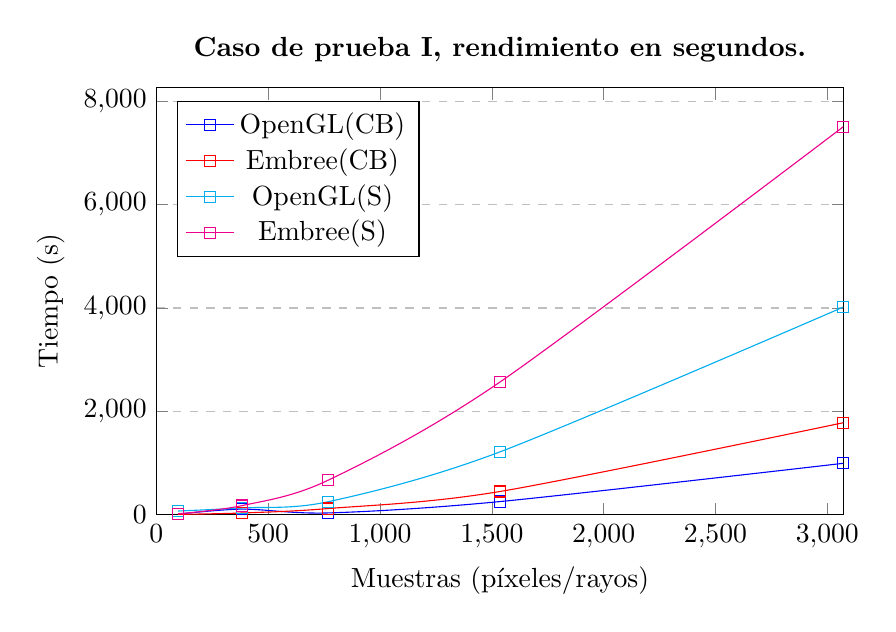
\begin{tikzpicture}
\label{plot:emglc1}
\begin{axis}[
title={\textbf{Caso de prueba I, rendimiento en segundos.}},
xlabel={Muestras (píxeles/rayos)},
ylabel={Tiempo (s)},
xmin=0, xmax=3072,
ymin=0,
width=.85\textwidth, height=7cm,
legend pos=north west,
ymajorgrids=true,
grid style=dashed,
]

\addplot[
smooth,
color=blue,
mark=square,
]
coordinates {
	(96,7)(384,105)(768,31)(1536,251)(3072,992)
};
\addplot[
smooth,
color=red,
mark=square,
]
coordinates {
	(96,3)(384,30)(768,116)(1536,446)(3072,1778)
};

\addplot[
smooth,
color=cyan,
mark=square,
]
coordinates {
	(96,68)(384,128)(768,248)(1536,1213)(3072,4018)
};

\addplot[
smooth,
color=magenta,
mark=square,
]
coordinates {
	(96,14)(384,174)(768,665)(1536,2565)(3072,7511)
};

\legend{OpenGL(CB),Embree(CB),OpenGL(S), Embree(S)}

\end{axis}
\end{tikzpicture}

Una de las consecuencias más interesantes a ser analizadas para detectar la cantidad de muestras óptimas a considerar es la calidad de la imagen final, y qué tan pronunciados son las diferencias en de iluminación entre los parches, es decir, en qué medida difiere la radiosidad entre parches. Para este caso, se pudo observar (véase la figura \ref{img:difres}) que si bien las resoluciones más bajas consumen menor cantidad de recursos los resultados tienen una calidad sustancialmente menor a la esperada. Considerando que el modelo generalmente es utilizado para el cálculo de mapas de iluminación en una etapa de pre-procesado, es recomendable evitar el uso de factores de muestreo tan bajos. Esto se ve acentuado en el análisis de la matriz de factores de forma, según las métricas establecidas en \ref{metricasestablecidas} se pudo comprobar que máximo error promedio apreciado (medida que se ha denominado $Ep$) fue de $4.15 10^{-5}$ y $3.91 10^{-5}$ utilizando $1536$ muestras para los métodos del hemicubo y la hemiesfera mientras que el uso de $96$ muestras generó errores del entorno de los $3.10 10^{-3}$ y $8.52 10^{-4}$ respectivamente. Estos errores se ven aún más acentuados al realizar el calcular la radiosidad para cada parche.

\begin{figure}[H]
	\centering
	\begin{subfigure}{0.45\textwidth}
		\includegraphics[width=1\linewidth]{assets/32sgl}
		\caption{OpenGL - 32 píxeles por cara}
	\end{subfigure}
	\begin{subfigure}{0.45\textwidth}
		\includegraphics[width=1\linewidth]{assets/512sgl}
		\caption{OpenGL - 512 píxeles por cara}
	\end{subfigure}
	\begin{subfigure}{0.45\textwidth}
		\includegraphics[width=1\linewidth]{assets/32srt}
		\caption{Embree - 96 rayos}
	\end{subfigure}
	\begin{subfigure}{0.45\textwidth}
		\includegraphics[width=1\linewidth]{assets/512srt}
		\caption{Embree - 1536 rayos}
	\end{subfigure}
	\caption{Diferencias visuales ajustando la cantidad de muestras}
	\label{img:difres}
\end{figure}

\subsubsection{Caso de prueba I}
  \chapter{Conclusiones y trabajo futuro}
\label{ch:chap06}

Este capítulo presenta las conclusiones principales en relación a la investigación realizada sobre el modelo de iluminación global implementado y sus extensiones para considerar superficies especulares, junto a un conjunto de posibles líneas de trabajo para extender los algoritmos implementados.

\section{Conclusiones}
\label{sec:conclusiones}

Este proyecto se dedicó al estudio, adaptación, implementación, extensión y comparación de distintos modelos de iluminación global que han surgido durante los años basados el método de radiosidad, así como posibles estrategias que optimicen el tiempo de ejecución observado.

En este sentido, se logró comprobar que las extensiones del método de radiosidad que toman en consideración el fenómeno de la reflexión difusa logran resultados con mayor realismo observándose un costo adicional de computación negligible, sobre todo al utilizar la técnica de traza de rayos.

Adicionalmente, se comprobó que el método del hemicubo comúnmente usado en la técnica no presenta buenas características para ser integrado en el cálculo de los factores de forma extendidos. Sino que el hecho de recurrir a métodos auxiliares para computar las direcciones de rebote son aproximaciones que pueden degradar la calidad de los resultados. No obstante, el método se muestra superior en escenas exclusivamente difusas aún cuando no se han implementado estructuras de aceleración para el cálculo.

En lo que refiere a la interfaz de usuario y las funcionalidades auxiliares implementadas se ha podido comprobar que fueron de utilidad para facilitar la ejecución y diseño de las pruebas permitiendo la exportación e importación de los datos obtenidos de forma sencilla y genérica. El uso de formatos estandarizados fue sin lugar a dudas una elección que enriqueció la usabilidad del programa.

Sobre las distintas tecnologías utilizadas se destaca la facilidad de manejo de la geometría en Embree como a su vez la flexibilidad de su uso utilizando bibliotecas de manejo de hilos como OpenMP. Además, se destacan las distintas extensiones de OpenGL que hicieron posible el uso de \textit{compute shaders} para reducir los hemicubos proyectados a filas de la matriz de factores de forma y la simpleza del uso de \textit{geometry shaders} y arreglos de texturas para reducir al mínimo los costos de las mutaciones del estado en lo que respecta de \textit{render targets}.

Finalmente se destaca el uso de la metodología \textit{Kanban} para el control y seguimiento de requerimientos y tareas; junto al uso de programación orientada a objetos para abstraer los conceptos y ofrecer una capacidad mayor de re-utilización de componentes y extensión de los métodos, como por ejemplo la clase \textit{Pipeline} concebida exclusivamente para superficies difusas utilizando OpenGL para luego extenderla de forma tal que se incluyeran métodos de traza de rayos con Embree y extensiones de los algoritmos de cálculo de factores de forma. 

\section{Trabajo futuro}
\label{sec:futuro}

Este proyecto puede ser continuado en distintas líneas de trabajo que fueron surgiendo a lo largo de la implementación y estudio de las soluciones desarrolladas.

En primer lugar, sería de gran interés la adición de estructuras de aceleración en OpenGL como por ejemplo, el uso de \textit{octrees}. Estas estructuras arborescentes permiten el descarte de dibujado de ciertas agrupaciones de primitivas a nivel de CPU y por tanto eliminan el costo del cálculo del algoritmo del Z-Buffer en gran medida. Además, sería beneficioso investigar la posible implementación del \textit{renderer} de OpenGL en la API Vulkan, en esencia esta API ha sido optimizada para minimizar el impacto del controlar de la GPU en la CPU, además provee facilidades que permiten enviar comandos de dibujado desde distintos hilos, lo que disminuiría la necesidad de sincronización entre el controlador de pre-procesamiento (\textit{PreprocessorController}) y la el controlador del dispositivo.

Por otro lado, sería beneficioso implementar un \textit{plugin} de la con los algoritmos implementados para \textit{software} de terceros, como por ejemplo el programa \textit{Blender}, que se ha utilizado para editar los objetos 3D en las escenas de prueba aunque provee de funcionalidades que calculan la iluminación global. Además, como se aprecia en la figura \ref{img:text} el uso de texturas proporciona detalles visuales que enriquecen la imagen generada, aunque la técnica de radiosidad es utilizada para el cálculo de la iluminación, es decir, es una de las etapas necesarias para generar imágenes fotorealistas.

\begin{figure}[H]
	\centering
	\includegraphics[width=.7\linewidth]{assets/text}
	\caption{Ejemplificación de la adición de texturas a los objetos de la escena}
	\label{img:text}
\end{figure}

Finalmente, el desarrollo de nuevo \textit{hardware} permite la que traza de rayos pueda ser acelerada por la GPU, por ello se propone el análisis de los algoritmos implementados en este tipo de dispositivos.

  \listoffigures	        
  \listoftables	         	
  
  \backmatter 
  

  \bibliography{bibliography} 
  \bibend

  
\end{document}

% ===== FIN DEL DOCUMENTO =====

